% File tacl2018v2.tex
% Sep 20, 2018

% The English content of this file was modified from various *ACL instructions
% by Lillian Lee and Kristina Toutanova
%
% LaTeXery is mostly all adapted from acl2018.sty.

\documentclass[11pt,a4paper]{article}
\usepackage{times,latexsym}
\usepackage{url}
\usepackage[T1]{fontenc}

%% Package options:
%% Short version: "hyperref" and "submission" are the defaults.
%% More verbose version:
%% Most compact command to produce a submission version with hyperref enabled
%%    \usepackage[]{tacl2018v2}
%% Most compact command to produce a "camera-ready" version
\usepackage[acceptedWithA]{tacl2018v2}
%% Most compact command to produce a double-spaced copy-editor's version
%%    \usepackage[acceptedWithA,copyedit]{tacl2018v2}
%
%% If you need to disable hyperref in any of the above settings (see Section
%% "LaTeX files") in the TACL instructions), add ",nohyperref" in the square
%% brackets. (The comma is a delimiter in case there are multiple options specified.)

% \usepackage[]{tacl2018v2}




%%%% Material in this block is specific to generating TACL instructions
\usepackage{xspace,mfirstuc,tabulary}
\newcommand{\dateOfLastUpdate}{Sept. 20, 2018}
\newcommand{\styleFileVersion}{tacl2018v2}

\newcommand{\ex}[1]{{\sf #1}}

\newif\iftaclinstructions
\taclinstructionsfalse % AUTHORS: do NOT set this to true
\iftaclinstructions
\renewcommand{\confidential}{}
\renewcommand{\anonsubtext}{(No author info supplied here, for consistency with
TACL-submission anonymization requirements)}
\newcommand{\instr}
\fi



% Standard package includes
\usepackage{times}
\usepackage{latexsym}
\usepackage{amsmath}
% For proper rendering and hyphenation of words containing Latin characters (including in bib files)
\usepackage[T1]{fontenc}
% For Vietnamese characters
% \usepackage[T5]{fontenc}
% See https://www.latex-project.org/help/documentation/encguide.pdf for other character sets

% This assumes your files are encoded as UTF8
\usepackage[utf8]{inputenc}

% This is not strictly necessary, and may be commented out,
% but it will improve the layout of the manuscript,
% and will typically save some space.
\usepackage{microtype}

% If the title and author information does not fit in the area allocated, uncomment the following
%
%\setlength\titlebox{<dim>}
%
% and set <dim> to something 5cm or larger.

\usepackage{soul} % colors

% own packages
\usepackage{graphicx} % figures
% \usepackage{float}
\usepackage{subfig} % for subfloats
% \usepackage[caption=false]{subfig}
\usepackage{booktabs} % nice tables
\usepackage{multirow} % multi column
\usepackage{comment} % for commenting text
\usepackage{amssymb} % check mark
\usepackage{multicol}
\usepackage{dsfont} % math
\usepackage[shortlabels]{enumitem} % letters enumeration



%
\iftaclpubformat % this "if" is set by the choice of options
\newcommand{\taclpaper}{final version\xspace}
\newcommand{\taclpapers}{final versions\xspace}
\newcommand{\Taclpaper}{Final version\xspace}
\newcommand{\Taclpapers}{Final versions\xspace}
\newcommand{\TaclPapers}{Final Versions\xspace}
\else
\newcommand{\taclpaper}{submission\xspace}
\newcommand{\taclpapers}{{\taclpaper}s\xspace}
\newcommand{\Taclpaper}{Submission\xspace}
\newcommand{\Taclpapers}{{\Taclpaper}s\xspace}
\newcommand{\TaclPapers}{Submissions\xspace}
\fi

%%%% End TACL-instructions-specific macro block
%%%%

\definecolor{WildStrawberry}{HTML}{ffab91}
\definecolor{OrangeRed}{HTML}{ff7043}

\definecolor{LightBlue}{HTML}{98F5FF}


\DeclareRobustCommand{\hltrue}[1]{{\sethlcolor{LightBlue}\hl{#1}}}
\DeclareRobustCommand{\hlfalseo}[1]{{\sethlcolor{pink}\hl{#1}}}
\DeclareRobustCommand{\hlfalset}[1]{{\sethlcolor{WildStrawberry}\hl{#1}}}
\DeclareRobustCommand{\hlfalsetr}[1]{{\sethlcolor{OrangeRed}\hl{#1}}}


% \DeclareRobustCommand{\hlgray}[1]{{\sethlcolor{lightgray}\hl{#1}}}
\DeclareMathOperator*{\argmin}{argmin}
\DeclareMathOperator*{\argmax}{argmax}


\newcommand{\ye}[1]{\textcolor{purple}{Yanai: #1}}
\newcommand{\sr}[1]{\textcolor{blue}{Shauli: #1}}
\newcommand{\nk}[1]{\textcolor{brown}{Nora: #1}}
\newcommand{\ar}[1]{\textcolor{magenta}{Lasha: #1}}
\newcommand{\hs}[1]{\textcolor{orange}{Hinrich: #1}}
\newcommand{\yg}[1]{\textcolor{purple}{Yoav: #1}}
\newcommand{\am}[1]{\textcolor{red}{[Amit: #1]}}

\newcommand{\resource}{\textsc{ParaRel}\raisebox{-2pt}{
\includegraphics[width=0.15in]{figures/horns}}}
% \newcommand{\resource}{\textsc{ParaRel}}

\newcommand{\subj}{\textit{X}}
\newcommand{\obj}{\textit{Y}}

\newcommand{\yenew}[1]{\textcolor{purple}{#1}}

\title{Measuring and Improving Consistency in Pretrained Language Models}


% Author information does not appear in the pdf unless the "acceptedWithA" option is given
% See tacl2018v2.sty for other ways to format author information
% \author{
%  Template Author\Thanks{The {\em actual} contributors to this instruction
%  document and corresponding template file are given in Section
%  \ref{sec:contributors}.} \\
%  Template Affiliation/Address Line 1 \\
%  Template Affiliation/Address Line 2 \\
%  Template Affiliation/Address Line 2 \\
%   {\sf template.email@sampledomain.com} \\
% }

 \author{Yanai Elazar\textsuperscript{1,2} \,
 Nora Kassner\textsuperscript{3} \,
 Shauli Ravfogel\textsuperscript{1,2} \, 
 Abhilasha Ravichander\textsuperscript{4} \, \\
 {\bf Eduard Hovy\textsuperscript{4}\, 
 \bf Hinrich Sch\"utze\textsuperscript{3}\, 
 Yoav Goldberg\textsuperscript{1,2}}\\
\textsuperscript{1}Computer Science Department, Bar Ilan University \\
\textsuperscript{2}Allen Institute for Artificial Intelligence \\
\textsuperscript{3}Center for Information and Language Processing (CIS), LMU Munich\\
\textsuperscript{4}Language Technologies Institute, Carnegie Mellon University \\
  {\tt  \{yanaiela,shauli.ravfogel,yoav.goldberg\}@gmail.com}\\
  {\tt kassner@cis.lmu.de} 
  {\tt \{aravicha,hovy\}@cs.cmu.edu} 
  }
 

\date{}

\newcounter{notecounter}
\newcommand{\enotesoff}{\long\gdef\enote##1##2{}}
\newcommand{\enoteson}{\long\gdef\enote##1##2{{
\stepcounter{notecounter}
{\large\bf
\hspace{1cm}\arabic{notecounter} $<<<$ ##1: ##2
$>>>$\hspace{1cm}}}}}
\enoteson
%\enotesoff

\begin{document}
\maketitle

\begin{abstract}
%We study consistency in Pretrained Language Models (PLMs),
%with respect to factual knowledge.

\textit{Consistency} of a model --- that is, the invariance
of its behavior under meaning-preserving alternations in its
input --- is a highly desirable property in natural language
processing.  In this paper we study the question: Are
Pretrained Language Models (PLMs) consistent with respect to
factual knowledge?\ar{Should we make this question less
binary- "and if not, to what extent are they consistent"}
\enote{hs}{my preference would be to keep it simple and
short in the abstract and explain the whole complexity of
the problem in the body of the paper}
To this end, we create \resource{}, a
high-quality resource of cloze-style query English
paraphrases. It contains a total of 328 paraphrases for thirty-eight relations. Using \resource{}, we show that the consistency
of all PLMs we experiment with is poor -- though with high
variance between relations.  Our analysis of the
representational spaces of PLMs suggests that they have a
poor structure and are currently not suitable for
representing knowledge in a robust way.  Finally, we propose
a method for improving model consistency and experimentally
demonstrate its effectiveness.

\end{abstract}


% \section{Introduction}
\label{sec:intro}

Pretrained Language Models (PLMs) have become popular in recent years and are used in many NLP tasks and applications.
An ongoing line of research is to understand how these models work, and analyzing what they can and cannot do.
For example, previous work showed that PLMs are very successful at capturing syntax, as was shown both in behavioral probes \cite{yoav-syntax} and structural probes \cite{structural-probe}.
On the other hand, other capabilities such as reasoning \cite{talmor2019olmpics}, commonsense \cite{Bosselut2019COMETCT,zhou2020evaluating} and world knowledge \cite{lama,jiang2020can} are moderate, and it has been questioned if these can be captured solely by PLMs at all \cite{Bender2020ClimbingTN}.


More recently, PLMs were suggested to be used as strong baselines for Knowledge Bases \cite{lama,jiang2020can}. Although the results of these models in the zero-shot setting outperform some supervised baselines, the results are still low, and the setup is limited (e.g. only reconstructing objects that consist of a single token, or the inability to return more than a single answer, or no answer whatsoever).
Yet, these studies lack an even more important property of KBs, that is \textit{consistency} and \textit{determinism}.
% \nk{I would add in this place a definition of the two terms}
% These properties require that the results returned from queries that are mapped into the same query in a KBs, will return the same results and in the same order.  
If two queries $q_1$ and $q_2$ are equivalent in the KB (e.g., if $q_1$ and $q_2$ are two equivalent ways to ask, in the formal language specified by the KB, for the retrieval of US presidents), they should return the same results, in the same order.
For example, consider the statement ```Homeland' was released on [MASK]'', where the `[MASK]' is the masked token that the model has to predict. We expect a model to predict the same answer with a pattern entailed by it: ``Homeland was aired on [MASK]'', e.g. \textit{Showtime}.
Note that in consistency, we do not expect the answers to be correct in the real world, which is a separate problem and has been addressed before, but for the predictions to be consistent, regardless of their true value.
These properties, although standard and well studied in classic KBs \cite{hansen2000probabilistic,Thimm:2009d,muino2011measuring}, are important for automatically constructed KBs.
% However, these properties were not studied in the context of LMs. 
However, it has not been studied to what extent PLMs used as KBs fulfill these requirements.
We note that consistency is largely \emph{independent} of accuracy, which is the property often studied: an inaccurate model can still err consistently, and it is possible that a specific PLM that is used as KBs is accurate \emph{only provided} it is queried in the ``correct" way, thus showing inconsistency when it is being used with semantically-equivalent natural-language queries.
Finally, these properties are important not only in the KBs usage, but in many other applications, such as Question Answering, Textual Entailment, etc, and was recently been addressed in the QA domain \cite{consistent-qa}. 


\begin{figure}[t!]
\centering

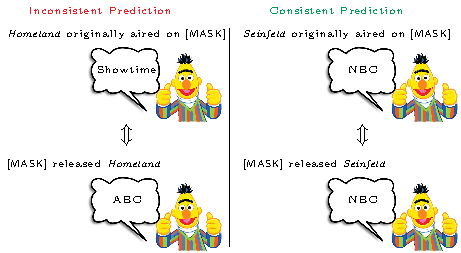
\includegraphics[width=1.\columnwidth]{figures/overview}

\caption{Overview of our approach. We begin with KB triplets (subject, pattern, object), of which we feed the (subject, pattern, [MASK]) into a PLM. 
We expect that a consistent model would predict the same answer for every two tuples of $(subject, pattern_1)$, $(subject, pattern_2)$ with an entailment connection between them. \nk{we should not use entailment but paraphrase connection right?}}
\label{fig:overview}
% \vspace{-6mm}
\end{figure}




In this work, we propose a new benchmark to test consistency in LMs, using factual knowledge that was claimed to be partially encoded in PLMs.
This benchmark includes a manually curated resource, that provides sets of similar patterns -- short textual prompts that describe some relation \sr{similar in what sense?}.
Then, expecting from consistent models to predict the same answer for every two patterns with an entailment edge. \sr{the term ``entailment edge" is undefined at this point. Further, it is not clear what entailment even mean at this point in the intro.}
% We do so by conditioning on some factual knowledge statements that are stored by the model (the premise), and test whether the model correctly predict an inferred statement (the hypothesis).
An overview of our approach is displayed in Figure \ref{fig:overview}.




In order to test these capabilities, we manually build an Entailment Graph \cite{berant2011global,berant2012global,javad2018learning,hosseini2019duality} for each of the 41 relations in the T-REx dataset \cite{trex} provided by LAMA \cite{lama}, such as: \textit{born-in}, \textit{is-a-citizen}, \textit{works-for}, etc. 
These graphs were built by experts, and provide a high-quality resource, which we name \resource{}.
% \nk{jump from one graph to multiple graphs} 
Each of these graphs contains between @@-@@ different nodes, where each node is a pattern, e.g. ``[X] was aired on [Y]'', where \textit{[X]} and \textit{[Y]} are slot fillers for a subject and object.
These graphs are directional, which represent the entailment direction between two patterns (e.g. ``[X] was premiered on [Y]'' entails ``[X] was aired on [Y]'', but not the other way around).
Moreover, each edge is also annotated with the modification type (e.g. syntactic or lexical). %\nk{do we need to talk about syntactic and lexical here}.
% Moreover, the graphs also con the type of inference, such as lexical inference or syntactic inference \sr{I don't know re the term ``syntactic/lexical inference". Maybe focus on the alternations: ``we annotate the alternations between any pair of patterns as syntactic or lexical".}, which allows us to test different kinds of inference capabilities.
Examples of edges of the graphs are displayed in Table \ref{tab:rel-graph-examples}.



% Our framework \nk{the distinction between our data and the introduced framework is not clear here.} enables to test for consistency across different types of alternations in PLMs \nk{alternation is very vague}, and in this work, enabled by \resource{} we test for two prominent and basic capabilities: consistency over lexical and syntactic alternations. However, the framework is more general and allows to test other types of inferences, such as commonsense, pragmatics, etc. %\ar{Where is the boundary between lexical inference and commonsense inference}
% Moreover, by dissecting the consistency of PLMs, we provide a method to disentangle their inference capabilities, with those which are learned during training on some inference dataset, for instance, MNLI \cite{mnli}. 
% This will allow to better understand what kinds of capabilities a model learns during the pretraining step, and what it learns from a finetuning dataset. \sr{this sentence is redundant}
By evaluating the zero-shot consistency properties of models, we also allow inspecting these capabilities out-of-the-box, without adding finetuning biases. This allows to better understand what kinds of consistencies a model learns during pretraining, and will allow to track and improve this property in future work.


% By combining the \resource{} with the proposed framework, we are able to test different PLMs and how strong their consistency capabilities are.
Using \resource{}, we are able to probe for consistency in multiple PLMs.
We find that overall, current models perform poorly on the consistency benchmark, although there is a high variance between the different relations. 

Finally, we propose a method to boost the consistency capabilities of models, by continuing the pretraining with an additional consistency loss. Our results show promising results and achieve better consistency performance, but there's still a big gap before achieving consistent models.

\section{Introduction}
\label{sec:intro}

Pretrained Language Models (PLMs) are
large neural networks that are
used in a wide variety of NLP tasks. They operate under a
pretrain-finetune paradigm: models are first \emph{pretrained} over a large text corpus and then \emph{finetuned} on a downstream task. PLMs are thought of as good language encoders, supplying basic language understanding capabilities that can be used with ease for many downstream tasks.

A desirable property of a good language understanding model
is \emph{consistency}: the ability of  making consistent
decisions in semantically equivalent contexts, reflecting a
systematic ability to generalize in the face of language variability.

%the ability to make consistent decisions, reflecting a systematic generalization ability to understand language, regardless of language variability. \sr{not so clear} %\sr{This sense of ``consistency" focuses on the ability to reason in a way that is invariant to meaning-preserving alternations. Note this differs from the way we initially thought about consistency: a model that always predicts the same answer is also ``consistent" but surely doesn't express this meaning of consistency. It's ok to focus on the meaning we focus on here, but if we do so, shouldn't we focus in the experiments on cases where the model initially predicted correctly? our current evaluation doesn't align, to my understanding, with this definition in the intro.}.  \ar{The definition of inconsistency in my mind, is having beliefs that result in a contradictions. The paraphrase thing is one way to test this for some applicable relations (if you believe 'X was born in Paris' and 'The birthplace of X is Delhi', this results in a contradiction). We can make this clearer.} 
Examples of consistency include: predicting the same answer in reading comprehension tasks regardless of paraphrase \cite{consistent-qa}; making consistent assignments in coreference resolution \cite{denis2009global,chang2011inference}; or making summaries factually consistent with  the original document \cite{kryscinski2020evaluating}.
While consistency is important in many tasks, nothing in the
training process explicitly targets it. One could hope that
the unsupervised training signal from large corpora
made available to PLMs such as BERT or RoBERTa
\cite{bert,roberta} is sufficient to induce consistency and
transfer it to downstream tasks.
%This property is important for many tasks involving language and is hard to obtain solely in a locally supervised setting. \sr{what is locally supervised? how do we know it's hard?} 
% Ideally, a PLM such as BERT or RoBERTa \cite{bert,roberta} would arrive with such capability, persist during the finetuning step and allow the new model to make consistent predictions. 
%Ideally, a PLM such as BERT or RoBERTa \cite{bert,roberta} would learn such capability during the pretraining phase and then transfer it to the downstream task. \sr{I'd present it as a question: is the unsupervised pre-training signal enough to \emph{induce} consistency?} 
In this paper, we show that this is not the case.
%\ar{I think we can be more explicit here of how consistency can act as evidence of a more general and systematic ability to understand language.}


\begin{figure}[t!]
\centering

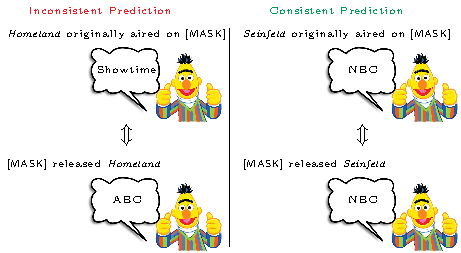
\includegraphics[width=1.\columnwidth]{figures/overview}

\caption{Overview of our approach. We begin with KB tuples (\textit{subject}, \textit{object}), of which we fill into a relational \textit{pattern} the: (\textit{subject}, \textit{[MASK]}) tuple,
% \nk{() are off here, also not sure if "populated" pattern is clear. Maybe also mention that the pattern is an relational pattern.}, 
and feed it into a PLM. 
We expect that a consistent model would predict the same answer for every two patterns $pattern_1$, $pattern_2$ which are paraphrases. 
In the example above, the model makes an inconsistent prediction for the left part of the figure and a consistent prediction on right part, where the subject is different.}
\label{fig:overview}
% \vspace{-6mm}
\end{figure}


The recent rise of PLMs has sparked a discussion about whether these models can be used as Knowledge Bases (KBs) \cite{lama,petroni2020how,alpaqa,roberts2020much}. 
% \nk{I would also cite this one maybe: "How Much Knowledge Can You Pack Into the Parameters of a Language Model?"}. 
Consistency is a key property of KBs and is particularly important for automatically constructed KBs.
%However, an important property of KBs, especially in automatically constructed KBs, is consistency.
One of the biggest appeals of using a PLM as a KB is that we can
query it in natural language -- instead of relying on a specific schema.
The expectation is that PLMs abstract away from language and map queries in natural language into meaningful representations such that queries with identical intent but different language form yield the same answer. 
For example, the query ``\textit{Homeland} was released on [MASK]'' should produce the same answer as ``\textit{Homeland} was originally aired on [MASK]''.
Studying inconsistencies of PLM-KBs can also teach us about the organization of knowledge in the model or lack thereof. 
Finally, failure to behave in a consistent manner may point
to other representational issues
% \nk{other issues seems a bit vague. Which other ones beside antonyms and synonyms do you have in mind?},
such as the similarity between antonyms and synonyms
\cite{nguyen2016integrating}.
% , symmetricity of the representation \enote{hs}{explain symmetricity, give citation} and the inability to handle negation. \nk{there was a paper studying this in PLMs right. Shouldn't we cite that one here}

% \ar{should we say "consistency of factual knowledge in PLMS through invariance to paraphrasing? This sentence makes it seem to me that consistency is equivalent to invariance to paraphrasing, but I think consistency is a broader problem. }
% \ar{Can we change the binary question here. "Is the" -> "to what extent"}
In this work, we study the consistency of factual knowledge
in PLMs: Is the factual information we extract from PLMs
invariant to paraphrasing? We use zero-shot evaluation since
we want to inspect models directly, without adding biases
through finetuning. This allows us to assess how
much consistency was acquired during pretraining and to
compare the consistency of different models.

%\sr{what does ``progress" mean here?}. %\sr{Question: how do we separate between lack of consistency due to the extraction method (maybe other extraction method would yield more consistent predictions), and an inherent lack of consistency in the model's behavior?}


We introduce \resource{}, a new benchmark  measuring
consistency in PLMs by using factual knowledge that was found to be partially encoded in them (\S \ref{sec:probe}).
\resource{} is a manually curated resource
that provides patterns -- short textual prompts -- that are paraphrases of one another, with 328 paraphrases describing thirty-eight binary relations such as \textit{X born-in Y}, \textit{X works-for Y} (\S \ref{sec:rel-graph}).
We then test multiple PLMs for knowledge consistency, i.e., whether
a model  predicts the same answer for all patterns of a relation.
Figure \ref{fig:overview} shows an overview of our approach.
Using \resource{}, we probe for consistency in four PLM
types: BERT, BERT-whole-word-masking, RoBERTa and ALBERT (\S
\ref{sec:setup}).
Our experiments with \resource{} show that
current models have poor consistency although there is a high variance between different relations (\S \ref{sec:experiments}). 

Finally, we propose a method that improves model consistency
by introducing a novel consistency loss
(\S \ref{sec:adding_consistency}). We demonstrate that models trained with this
loss achieve better consistency
performance on new relations. However, there still is much
work to do to achieve fully consistent models.

% Extending upon previous work that showed that factual knowledge can be extracted to some degree \cite{lama,alpaqa}, we extend their proposed patterns that were used to extract that information, and manually write paraphrases to the original patterns.


% \resource{} contains 40 relations from the T-REx dataset \cite{trex} provided by LAMA \cite{lama}, such as: \textit{born-in}, \textit{is-a-citizen}, \textit{works-for}, etc (\S \ref{sec:rel-graph}).
% The paraphrases were built by experts, and provide a high-quality resource.
% \nk{jump from one graph to multiple graphs} 
% Each of these graphs contains between @@-@@ different nodes, where each node is a pattern, e.g. ``[X] was aired on [Y]'', where \textit{[X]} and \textit{[Y]} are slot fillers for a subject and object.
% Moreover, each edge is also annotated with the modification type (e.g. syntactic, lexical) \sr{I am not sure we need to mention these in the intro, given the pretty narrow / heuristic way we define those}.
% Examples of edges of the graphs are displayed in Figure \ref{fig:graph}.


%%%%%%%%%%%%%%%


% By combining the \resource{} with the proposed framework, we are able to test different PLMs and how strong their consistency capabilities are.



% Jonathan:
% https://www.aclweb.org/anthology/P12-1013.pdf

% https://www.aclweb.org/anthology/P11-1062.pdf

% https://www.aclweb.org/anthology/P10-1124.pdf


% Mohammad Javad Hosseini:
% https://www.aclweb.org/anthology/P19-1468.pdf

% https://www.mitpressjournals.org/doi/pdfplus/10.1162/tacl_a_00250

% inference
% https://arxiv.org/pdf/1909.07521.pdf
% https://arxiv.org/pdf/2002.05867.pdf
% https://arxiv.org/pdf/2006.06609.pdf
% https://arxiv.org/pdf/2007.00655.pdf

\section{Background}
\label{sec:background}

There has been significant interest in analyzing the capabilities of PLMs \cite{rogers2020primer}, including linguistic tasks \cite{yoav-syntax,hewitt2019structural,tenney2019bert,amnesic_probing}, commonsense capabilities \cite{forbes2019neural, da2019cracking,zhang2020language} and ability to reason \cite{talmor2019olmpics, kassner-etal-2020-pretrained}. However, there has been considerably less research attention devoted to analyzing how \emph{consistent} models are on these abilities. That is, to what extent do such probes uncover generalizable capabilities of a model and how indicative are they of a coherent set of beliefs in the model. Some initial work in this area has shown that models can be equally prone to generating facts and their negation, a type of inconsistent behavior \cite{Ettinger_2020,kassner-schutze-2020-negated}. \newcite{ravichander-etal-2020-systematicity} propose consistency probes - paired probes to evaluate the ability of PLM to behave in a coherent manner. However, our work is broader in scope, examining the behaviour of PLMs across a range of factual knowledge types, and investigating how models can be made to behave more consistently. 

Consistency has also been highlighted as a desirable property in automatically constructed KBs and downstream NLP tasks, which we describe below:

\paragraph{Consistency in Knowledge Bases}

Consistency has been studied under theoretical frameworks in the contexts of the satisfiability problem and KBs constructions, and efficient algorithms that detect inconsistencies in KBs have been proposed \cite{hansen2000probabilistic,andersen2001easy}.
Other works, aim to quantify the degree to which KBs are inconsistent and detect the inconsistent statements \cite{Thimm:2009d,muino2011measuring,Thimm:2013}.



\paragraph{Consistency in Question Answering}
Consistency of models was studied in the Q\&A domain as well. \citet{ribeiro-etal-2019-red} studied the consistency capabilities of several models, in two Q\&A tasks: Visual Question Answering \cite{vqa} and Reading Comprehension \cite{squad}. They generate questions with an automatic method, that allows them to test the consistency of Q\&A models.
Their findings suggest that most models are not consistent in their predictions, and they also use data augmentation to create more robust models.
\citet{alberti2019synthetic} proposed to generate new questions conditioned on the context and answer from a labeled dataset, and by filtering answers that do not provide a consistent result with the original answer. The authors show that pretraining on this synthetic data improves the results on Q\&A datasets.
\citet{consistent-qa} proposed to use data augmentation that complements questions with symmetricity and transitivity, as well as a regularizing loss that penalizes inconsistent predictions.

\paragraph{Consistency in Other Domains}
Consistency was also studied in other domains. For example, \citet{du2019consistent} improves predictions consistency in procedural text over similar descriptions. \citet{ribeiro-etal-2020-beyond} uses consistency for more robust evaluation. \citet{li-etal-2019-logic} measure and mitigate inconsistency in natural language inference.

%\ar{We should add work examining consistency in PLMs - i.e negated lama, systematicity of probing cwr, }

% \section{Consistency Probing of Knowledge}
\section{Probing PLMs for Consistency}
\label{sec:probe}

In this section, we formally define consistency and describe
our framework for probing the consistency of PLMs.

\subsection{Consistency}
We define a model as \emph{consistent} if, given  two
\textit{cloze-phrases} such as 
 ``Seinfeld originally aired on [MASK]'' and
``Seinfeld premiered on [MASK]'' that
are \textit{quasi-paraphrases} it makes the same
prediction.\footnote{A \textit{quasi-paraphrase} --
  introduced by \citet{what_is_paraphrase} -- is a more
  fuzzy version of a paraphrase. The concept does not rely
  on the strict, logical definition of paraphrase and
  allows to operationalize concrete uses of
  paraphrases. This definition is in the spirit of the RTE
  definition \cite{dagan-rte}, which similarly supports a
  more flexible use of the notion of entailment.}
\enote{hs}{I don't understand what this sentence says
-- in  addition to what was previously already said:
  
In the context of PLM knowledge consistency, if two cloze-phrases 
% \yg{we didn't define cloze-phrases yet. do they include a relation tuple?} 
of some relation (e.g., \textit{originally-aired-on}) are quasi-paraphrases, masked language models should predict the same entity for the masked item. 
% \sr{I changed the wording here. Is it still what you meant? a natural question now is ``why objects".}
% \yg{can it be "masked item"? or is it really a syntactic
% object?}
}
In the rest of the paper, we use the terms \textit{paraphrase} and \textit{quasi-paraphrase} interchangeably.

 
\enote{hs}{following paragraph: this sounds like quite a big
  problem to me: isn't it a huge assumption that the order
  of prediction will be the same for all paraphrases? is
  this seomthing we woudl expect of human performance?

  Can we move this to a later point in the paper and say:
  this is something that we will investigate in the future?}
We note that this definition does not take into account the type (e.g., one-to-one or many-to-many) of the relation. %\yg{what relation? we didn't say relation in this secction until now.} 
For instance, some relations are defined as \textit{many-to-many}, and as such, more than a single item can be factually correct, even for quasi-paraphrases. However, we still expect that the order will remain, and thus even if the alternative answer is factually correct, we still consider cases with different answers as a non-consistent result.

\subsection{The Framework}
\label{sec:framework}
Let
$D = \{D_1, D_2,
\dots, D_m\}$
be a set of sets of KB triples,
where each $D_i$ contains factual statements
that express a specific relation $R_i$. In this section, we
us $R_1$ = ``premiered
on'' and $D_1$
as running example. Each $D_i=\{d_1^i,
d_2^i, \dots, d_n^i\}$
is composed of $n$ examples  where each $d_j^i = <s_j^i,o_j^i>$
is a subject-object tuple from the relation $R_i$. 
For example,
$<\text{\textit{Homeland}},
\text{\textit{Showtime}}>$
is an example of a 
tuple in $D_1$.
Each relation $R_i$ is associated with a set of
cloze-patterns $P_i$ that are \textit{quasi-paraphrases} of
each other, i.e., they express the same relation $R_i$. For example, $P_1=\{p_1^1, p_2^1, \dots, p_n^1\}$ contains the patterns ``\subj{} was originally aired on \obj{}'' and ``\subj{} premiered on \obj{}''.
\nk{I think we should have someone who is not familiar with our setup check this passage. I am not sure if everyone will understand it}
\yg{I agree, hard to follow. I propose to possible solutions: (1) start bottom-up rather than top-down: this is a pattern, here is a group of patterns, now we collect them into a set... (2) visualize it in a figure (instead of the text).}
\am{while I'm familiar with this work, reading this
  paragraph for the first time I can understand the
  definitions. I agree with Yoav that a visualization can
  help though}
\enote{hs}{I do think the reader has to put in a little bit
  of effort, but I'm the type of writer who expects that of
  the reader. I agree that we should consider a figure!}

Given some relation $R_i$, a subject-object tuple $d_j^i \in
D_i$ (e.g., `Homeland', `Showtime') and two paraphrases
$p_k^i, p_l^i \in P_i$ associated with this relation (such
as ``\subj{} was originally aired on \obj{}'' and ``\subj{}
premiered on \obj{}''), our goal is to test whether the
model consistently predicts the same object for a particular subject.
To this end, we
substitute \subj{} with a selected subject and \obj{} with
MASK; we write this as $p_k^i(s_j^i,mask)$,
$p_l^i(s_j^i,mask)$ or (for a specific example) as
``Homeland was originally aired on [MASK]'', ``Homeland was premiered on [MASK]''.
Finally, we extract the model's most probable prediction for
MASK in the two sentences.  A consistent model must predict the same entity. Note that the consistency measure does not require the answers to be factually correct. While correctness is also an important property for KBs, we view it as separate objective and measure it independently. 

% If the model predicts the correct $o_j^i$ as the most probable completion, we take that as evidence for the storing of the factual knowledge $d_j^i$ in the model. 
% In this case, a model that can perform adequate inference over the syntactic and lexical alternations between $p_j^i$ and $p_k^i$ is expected to also correctly predict the object from the alternative patterns $p_k^i$.

\paragraph{Restricted Candidate Sets}
Ideally, we would focus on the top-1 prediction that the PLM produces in order to compare between paraphrases. However, since these models were not trained for the purpose of serving as KBs, but as LMs, words outside of the inspected entities are often possible (e.g., the object in ``\subj{} was originally aired on \obj{}'' can also be replaced with `tv', to make a proper English sentence).
Therefore, we restrict the vocabulary produced by the PLMs to a candidate set, that is the set of possible gold objects for each relation, as was also suggested in previous work \cite{Xiong2020Pretrained, nora@@}.

Note that this procedure is a relaxation of the general problem, especially in the context of KBs, however, low consistency results in this setup are even more alarming.


\section{The \resource{} Resource}
\label{sec:rel-graph}

We now describe \resource{}, a concrete resource according to the framework described in Section \ref{sec:framework}.
% To measure PLMs' consistency, we test their predictions sensitivity to various paraphrased queries. 
% We create a paraphrase resource that enables us to study this property, which we name \resource{}. \am{last 2 sentences are redundant. keep only the first imo} \resource{} is a high-quality resource, built by experts. %, and results in a high-quality resource which we hope can contribute to others' work as well.
\resource{} is a high-quality resource, built by experts.
It contains patterns for thirty-eight relations from the T-REx dataset \cite{trex}, with an average of 8.63 patterns per relation.
Some statistics of the resource are presented in Table \ref{tab:rel-graph-stats}.

% Each pattern is represented as a node in an undirected graph, and each edge signifies the type of modification from one pattern to another (e.g. lexical change).
% A schematic view of the ``aired on'' relation can be seen in Figure \ref{fig:graph}. 

% All patterns from a specific relation are paraphrases.
% Each pattern entails the main expression for each pattern, but not necessarily the other way around. 
% For example, for the relation of ``aired on'', which describes a TV-series that was aired on some network, the original pattern is: ``\subj{} was aired on \obj{}'' and one of the patterns we create is ``\subj{} was premiered on \obj{}'', which entails the main expression, but not vice versa.


% For instance, the phrase "\subj{} was aired on \obj{}" entails "\obj{} released \subj{}", but not "\subj{} was premiered on \obj{}", although the other direction is entailed.
% \ar{The entailment 'Y released X' doesn't seem correct. Suggestion For instance, the phrase "\subj{} was premiered on \obj{}" entails "\subj{} was aired on \obj{}", but not the other way around.}

% \begin{figure}[t!]
% \centering

% 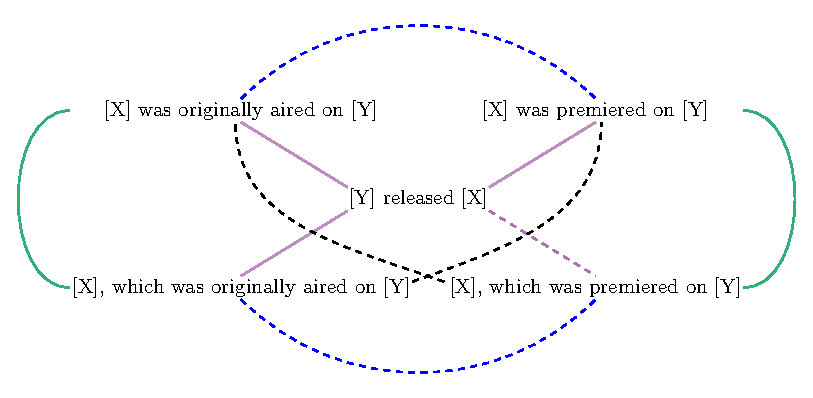
\includegraphics[width=1.\columnwidth]{figures/ent_graph}

% \caption{Overview of \resource{}.}
% \label{fig:graph}
% % \vspace{-6mm}
% \end{figure}

% Overall, \resource{} contains @@ different patterns in total for @@ different relations (@@\% paraphrases per relation in average). 
% All of the paraphrases for a particular relation are organized as a directed graph to indicate the entailment relation between two patterns. 
% Each edge also contains information about the transformation type, e.g. a lexical or syntactic transformation (Examples for each can be seen in Figure \ref{fig:graph}).
%A detailed definition is provided shortly.
% \ye{need to define this.} 
% This information allows us to study the different generalization capabilities of models.
% The nodes of the graph (which account for the phrases), also contain additional information about the number of times that the pattern appeared in Wikipedia, @@ more?. %\ar{will we still have the wikipedia info in the paper?}

\paragraph{Construction Method}
\resource{} was constructed in four steps. (1) We began with
the patterns provided by LAMA \cite{lama} (one pattern per
relation, referred to as ``base pattern"). (2) We augmented
each base pattern with other patterns that are paraphrases of
the base pattern. Some of these paraphrases are taken from
LPAQA \cite{alpaqa}. However, since LPAQA was
extracted automatically, many LPAQA patterns are not
correct paraphrases.
We therefore only include the subset of correct paraphrases in \resource{}.
(3) Using SPIKE
\cite{spike},\footnote{\url{https://spike.apps.allenai.org/}}
a search engine over Wikipedia sentencecs that supports
syntax-based queries, we searched for additional patterns
that appeared in Wikipedia and added them to 
\resource{}. Specifically, we searched for Wikipedia sentences
containing a  subject-object
tuple from T-REx and then manually extracted 
patterns from the  sentences. (4) Lastly, we added
additional patterns that are paraphrases of the base pattern
using the annotators' linguistic expertise.  Two additional
experts went over all the patterns and corrected them, while
engaging in a discussion until reaching  agreement,
discarding patterns they could not agree on.

% (The annotators can also add entailing or entailed patterns, but we do not make use of them in this paper.)

% \nk{should we give a number?}.\ye{I don't think it's necessary}

% \nk{Not sure if the details of this need to be in the main paper or can be moved to the appendix?} \sr{I support moving the technicalities to an appendix and focus here on the properties of the resources and how it is being used.}
% \ye{can decide when we have the full story}
%The entailment edges were also annotated by the same two authors that created the patterns.

\begin{table}[t]
% \small
    \centering
\begin{tabular}{lr}
\toprule
           stat &   values \\
\midrule
      n. graphs &    15 \\
   avg patterns &    19.73 \\
   min patterns &     9 \\
   max patterns &    37 \\
       n. edges &  4821 \\
 edge syntactic &     0.03 \\
   edge lexical &     0.87 \\
      edge both &     0.09 \\
\bottomrule
\end{tabular}
    \caption{Statistics for \resource{}. \ye{numbers are not updates with all the graphs}}
    \label{tab:rel-graph-stats}
\end{table}


% \paragraph{Consistency Types}
% % \nk{we should change inference types to consistency types} \ye{but the graph is in entailment graph}
% To study the consistency against syntactic and lexical variations of models, each edge is augmented with the type of changes performed to reach from one pattern to another. We account for three types of changes: (1) \textit{syntactic}, (2) \textit{lexical} and (3) \textit{determiner}, all binary variables that account for a change of the specific type between two patterns.
% \textit{Syntactic} structure is defined as the dependency path between the subject and the object in a given pattern, where the path includes the edge types. Two patterns are considered equal syntactically if the labeled paths are identical.
% \textit{Lexical} difference is defined by words difference between two patterns, excluding determiners, punctuation, and symbols. The addition or removal of a preposition does not count as a lexical change.
% \textit{Determiner} difference is considered when the patterns' determiners do not fully overlap.



% and full statistics per relation are presented in Table \ref{tab:rel-graph-stats-elaborate} in the Appendix.


\paragraph{Human Agreement}
To assess the quality of \resource{}, we run a
human annotation study.
For each relation, we sample up to
five paraphrases, comparing each of the new patterns to the base pattern that came with that resource, and which is assumed to correctly describe the relation.
By definition, two patterns that are paraphrases of the base pattern are also paraphrases of each other.

We populate the patterns with random subjects and objects from T-REx \cite{trex} and ask annotators if these sentences are paraphrases.
We also sample patterns from different relations to provide examples that are not paraphrases of each other, for control.
Overall, each task contains five patterns that are thought
to be paraphrases, and two that are not.\footnote{The
  control patterns contain the same subjects and objects, so
  that only the pattern (not its argument) can be used to
  solve the task.}
Overall, we collect annotations for 156 paraphrase candidates and 61 false paraphrases for control.

We asked graduate students in NLP to  annotate the pairs and collected one answer per pair.
Due to random errors in the annotations, for every question
that does not match our original label (either for
paraphrases or controls), we ask the annotators to relabel
them (without specifying the reason), to allow them to fix
random mistakes.\footnote{Moreover, due to the sampling of
  patterns from different relations, seldom the patterns may
  be paraphrases of one another, which we do not count as
  mistakes.}

% \nk{I would cut that last sentence}

The agreement score for the paraphrases and the control are: 95.5\% and 98.3\%, which are high and reassures \resource's quality.
We further went through the disagreements  %of the paraphrases 
and fixed any additional problem %that we agree with, 
to further improve the resource quality.
Examples of paraphrases are displayed in Table \ref{tab:predictions}. 
% \am{a bit odd to send the reader all the way to table 4, at this stage}
% \begin{table*}[t]
% \small
    \centering
\resizebox{1\textwidth}{!}{%
\begin{tabular}{llll}
\toprule
           Pattern & Base &  Entailed & Type \\
\midrule
% hi & byw & chao \\
      \textsc{Died-in} & \textsc{Subj} passed away in \textsc{Obj}. & $\Leftrightarrow$ \textsc{Subj} died in OBJ. & lexical \\
       & \textsc{Subj} was murdered at \textsc{Obj}. & $\Rightarrow$ \textsc{Subj} died in \textsc{Obj}. & lexical \& syntactic \\
       & \textsc{Subj} died at \textsc{Obj}. & $\Leftrightarrow$ \textsc{Subj} died in \textsc{Obj}. & lexical \\
       
       \midrule
       
       \textsc{Official-language} & \textsc{Obj} is the official language of \textsc{Subj}. & $\Leftrightarrow$ The official language of \textsc{Subj} is \textsc{Obj}. & syntactic \\
       & In \textsc{Subj} \textsc{Obj} is an official language. & $\Leftrightarrow$ The official language of \textsc{Subj} is \textsc{Obj}.	& \\
       
       \midrule
       
       \textsc{Located-in} & \textsc{Subj} is a county in \textsc{Obj}. & $\Rightarrow$ \textsc{Subj} is located in \textsc{Obj} . & lexical \& syntactic \\
       & \textsc{Subj} district, \textsc{Obj}.	& $\Rightarrow$ \textsc{Subj} is located in \textsc{Obj} . & lexical \& syntactic \\
       
       \midrule
       
       \textsc{Instrument} & \textsc{Subj} was a \textsc{Obj} player. & $\Rightarrow$ \textsc{Subj} plays \textsc{Obj}. & lexical \& syntactic \\
       & \textsc{Subj} played \textsc{Obj} . & $\Leftarrow$ \textsc{Subj} plays \textsc{Obj}. & tense \\
       & \textsc{Obj} sonatas of \textsc{Subj}. & $\Rightarrow$ \textsc{Subj} plays \textsc{Obj}. & lexical \& syntactic \\
       
\bottomrule
\end{tabular}
}
    \caption{Examples of patterns in the \resource{}.}
    \label{tab:rel-graph-examples}
\end{table*}

One of the disagreements with our annotation arised from the following paraphrases: ``Royal Dutch Football Association is a member of FIFA.'' and ``Royal Dutch Football Association is affiliated with the FIFA organization.''
Although these phrases are not paraphrases in the general case, we believe they are in our case with football association. Such disagreement may arise from the lack of specific domain knowledge, but also from inherent disagreement in this sort of annotation that may arise from inherent disagreements \cite{pavlick2019inherent} or from different construals \cite{trott2020re}, which were recently observed in NLI \cite{elazar2020extraordinary}.


\section{Experimental Setup}
\label{sec:setup}

\subsection{Models \& Data}
\label{setupdata}
We experiment with four PLM variants: BERT, BERT whole-word-masking
\cite{bert}, RoBERTa \cite{roberta} and ALBERT
\cite{albert}. For BERT, RoBERTa and ALBERT, we use a base and a large version.\footnote{For ALBERT we use the smallest and largest versions.}
% Additionally, we use the whole-word-masking version of BERT large, which was shown to perform well in multiple tasks \cite{talmor2019olmpics}.
In addition, we also report a majority baseline that always predicts the most common object for a specific relation. By definition, this baseline is perfectly consistent.

% \subsection{Data}


% To probe for consistency of PLMs we use cloze-style queries using a (subject, relation, object) triple from a KB. We then populate the subjects and objects from the KB into patterns for all triplets in $D$ from \resource{} to create the cloze-style queries; e.g, ``\subj{} was aired in \obj{}''. \subj{} is substituted with the subject and \obj{} with a masked token (e.g. `[MASK]'). \nk{not sure if this is a bit confusing as it is saying the same as earlier a bit differently}\yg{I agree. Don't repeat, and refer to prev description.}

We use knowledge graph data from T-REx \cite{trex}.\footnote{We discard three poorly defined relations from T-REx.} To make the results comparable across models, we remove objects that are not represented as a single token in all models'
vocabularies, to a total of 26,813 tuples.
%TODO - {add back for camera ready}\footnote{In a few cases, we filter entities from certain relations that contain multiple fine-grained relations to make our patterns compatible with the data.}
We further split the data into N-M relations of which we report the determinism results apart (seven relations), as well as the N-1 which we use for measuring consistency (thirty-one relations). 
% Moreover, some relations contain aggregated data of different types, which makes the original LAMA pattern sometimes obsolete as it does not fit the type (e.g. the tuple (`My Family', `sitcom') in the \textit{genre} relation, that mainly contains music-genre entities).\yg{the prev sentence is not clear}\am{I agree} In these cases, we manually filter these entities from our test set.
% We use the patterns from our resource \resource{}, described in the previous section. \am{use them for, what?}

% \enote{hs}{above: i don't understand the footnote}

\subsection{Evaluation}
\label{sec:eval}

%\ye{I think typed querying should be defined properly}
% Following prior work \cite{Xiong2020Pretrained, }: for each relation, we create a
% candidate set $\mathcal{C}$ and then predict
% $\arg\max_{c\in \mathcal{C}}p(c|q)$ where $p(w|q)$ is the probability
% that word $w$ gets predicted in query $q$. For most relations,
% there is only one valid entity type, e.g., country for the ``captical-of'' relation.
% We choose as $\mathcal{C}$ the set of all possible objects for a specific relation from the TREx dataset.
% The candidate set could also be obtained from an entity
% typing system
% (e.g., \cite{yaghoobzadeh-schutze-2016-intrinsic}), but this
% is beyond the scope of this paper.

Our consistency measure for a relation $r_i$ (\textit{Consistency}) is the
percentage of consistent predictions of all the pattern pairs
of that relation $p_k^i,p_l^i \in P_i$, for all the KB tuples
$d_j^i \in D_i$. Thus, for every KB tuple from the relation $r_i$ that contains $n$ patterns, we compare $n(n-1)/2$ pairs.
%adding this here: "corresponding to the relations."
%would imply that there are also members of D_i that
%do not correspond to the realtion. but that is not the case?

We also report \textit{Accuracy} metric, that is, the acc@1 of a model in predicting the correct object, using the original patterns from \citet{lama}. In contrast to \citet{lama}, we define it as accuracy of the top-ranked object from the candidate set of each relation.
Finally, we report \emph{Consistent-Acc}, a new metric that evaluates individual objects as correct, only
if \emph{all} patterns of the corresponding relation predict the object
correctly. \textit{Consistent-Acc} is a much stricter metric and combines the
requirements of both consistency (\textit{Consistency}) and factual correctness (\textit{Accuracy}).

% In all our metrics, we report the average results over all relations, which can be viewed as a macro average.

We report the average (unweighted) results over all relations, that is -- macro average.


\section{Experiments and Results}
\label{sec:experiments}


\begin{table*}[t]
% \small
    \centering
\resizebox{1\textwidth}{!}{%
\begin{tabular}{lllllllll}
\toprule
Models &       LAMA & Group-Score &    Succ-Pat &  Succ-Objs &  Know-Const &   Unk-Const &  Const-Objs & Consistency \\

\midrule
majority-baseline &  24.2+-20.7 &  24.2+-20.7 &  100.0+-0.0 &  24.9+-20.7 &  100.0+-0.0 &  100.0+-0.0 &  100.0+-0.0 &  100.0+-0.0 \\ \midrule
bert-base         &  44.1+-25.6 &  25.0+-25.5 &  100.0+-0.0 &  60.6+-23.5 &  61.4+-23.2 &  45.2+-20.6 &  32.5+-28.5 &  57.3+-22.3 \\
bert-large        &  45.6+-27.0 &  27.5+-27.6 &   99.7+-1.8 &  63.0+-25.2 &  62.4+-22.4 &  46.4+-18.5 &  34.2+-30.0 &  59.1+-21.5 \\
bert-large-wwm    &  45.4+-26.4 &  27.2+-27.6 &  100.0+-0.0 &  61.6+-23.2 &  62.6+-23.6 &  46.5+-18.7 &  33.8+-29.8 &  58.6+-22.7 \\ \midrule
roberta-base      &  36.7+-24.6 &  16.0+-19.8 &  100.0+-0.0 &  54.2+-24.5 &  53.3+-20.2 &  41.2+-15.3 &  21.7+-23.1 &  50.1+-18.4 \\
roberta-large     &  40.8+-26.1 &  21.3+-23.7 &  100.0+-0.0 &  58.5+-24.1 &  58.2+-21.1 &  44.4+-16.0 &  27.4+-25.6 &  54.8+-19.6 \\ \midrule
albert-base       &  29.9+-24.2 &  17.0+-22.2 &   99.7+-1.8 &  45.3+-25.7 &  56.1+-21.5 &  43.1+-18.0 &  25.1+-25.4 &  51.2+-19.8 \\
albert-xxlarge    &  39.5+-26.1 &  21.9+-25.7 &   99.7+-1.8 &  56.3+-25.8 &  56.7+-22.7 &  38.8+-14.7 &  26.8+-26.8 &  51.5+-21.1 \\
\bottomrule
\end{tabular}


}
    \caption{Consistency and knowledge results for the different models.}
    \label{tab:consistency_main}
\end{table*}

\subsection{Consistency}

The results for the different models are summarized in Table \ref{tab:consistency_main}.
% First, we report the average consistency results for all graphs, as describe in Section \ref{sec:eval}.
The last column (``Consistency'') shows the average results across all relations \yg{consider oredering the table columns in the order of their discussion}\am{I actually like it in the end, its easier to find in a glance}

The BERT-based models achieve higher scores over all the models\am{over the others, or the rest}. Moreover, there is a consistent improvement from the base to large\am{emph or quote 'base' and 'large'} versions of each model, although it is not always significantly \am{is there a significance test?} higher (e.g. 57.3\% to 59.1\% in BERT, and 50.1\% to 54.8\% in RoBERTa).
However, in contrast to many previous works that observed quantitative and qualitative improvements of RoBERTa-based models over BERT, in terms of consistency\am{comma} BERT is better than RoBERTa and ALBERT.\am{I would rephrase and say "BERT is more consistent than ...."}
Still, the overall results are remarkably low (59.1\% for the best model, \yg{meaning that out of XXX, YYY are ZZZ}), especially given the permissive evaluation that only looks at the candidate set.
We note that the results are highly variant between models and relations. For instance, the best performing model on the `capital of' relation achieves 94\%, whereas the best performing model on `owned by' is 44\%\am{is what? "achieves"?}. 
On the other hand, the models' performance on the `original language of film or TV show' relation, varies between 52\% and 90\% accuracy.
We report the full consistency results for each relation in the Appendix.

\begin{table}[t]
% \small
    \centering
\resizebox{1\columnwidth}{!}{%
\begin{tabular}{lrrr}
\toprule
Model&        Acc & Consistency & Consistent-Acc \\

\midrule
majority               &  23.1+-21.0 &  100.0+-0.0 &  23.1+-21.0 \\
\midrule
RoBERTa-med-small-1M &   11.2+-9.4 &  37.1+-11.0 &    2.8+-4.0 \\
\midrule
RoBERTa-base-10M     &  17.3+-15.8 &  29.8+-12.7 &    3.2+-5.1 \\
RoBERTa-base-100M    &  22.1+-17.1 &  31.5+-13.0 &    3.7+-5.3 \\
RoBERTa-base-1B      &  \textbf{38.0}+-23.4 &  \textbf{50.6}+-19.8 &  \textbf{18.0}+-16.0 \\
\bottomrule
\end{tabular}
}
    \caption{Knowledge and consistency results for the different RoBERTas, trained on increasing amounts of data. Best model for each metric is highlighted in bold.}
    \label{tab:robertas}
\end{table}

% \enote{hs}{below: i would prefer ``(training) corpus size''
%   over ``number of tokens'' if that's what you mean}

\paragraph{Effect of Pretraining Corpus Size}
Next, we study the question of whether the number of tokens used during the pretraining contributes to consistency.
We use the pretrained RoBERTas model provided by \citet{robertas} and repeat the experiments on four additional models.
These models are RoBERTa-based models, that were trained on a sample of Wikipedia and the book corpus, with varying training size, and parameters. In practice, we use one of the three published models for each configuration and report the average accuracy over the relations for each model in Table \ref{tab:robertas}.
Overall, the consistency and the knowledge scores (LAMA and Group-Score) improve when trained on more data. \nk{Maybe I missed it, did we say what the Group-Score is before?}\am{seems like not} However, there is an interesting outlier to this trend.
First, the model that was trained on one million tokens is more consistent than the models trained on ten and one-hundred million tokens. A potentially crucial difference is that this model is also smaller in terms of the number of parameters than the rest, in order to avoid overfitting. Still, it is nonetheless interesting that a model that is trained on significantly fewer\am{I would use "less"} data can achieve better consistency. On the other hand, the knowledge scores are lower, arguably due to less factual knowledge this model was exposed to during training.\am{due to the model being exposed to less factual knowledge during pretraining}

% Finally, the original RoBERTa that was trained on ten billion parameters, achieves the same consistency performance as the one trained on one billion tokens, suggesting a limit to the benefit of training examples in pretraining. \nk{not sure about this as the table is not there yet, but shouldn't it be: Finally, the original RoBERTa that was trained on ten billion tokens, achieves the same consistency performance as the one trained on one billion tokens, suggesting on a limit to the benefit of large training corpora. }



% \begin{table*}[t]
% \small
    \centering
\resizebox{1\textwidth}{!}{%
\begin{tabular}{lrrrrrrr}
\toprule
{} &  bert-base &  bert-large &  bert-large-wwm &  roberta-base &  roberta-large &  albert-base &  albert-xxlarge \\
\midrule
syn   &             0.50 &              0.53 &                                 0.53 &          0.44 &           0.48 &            0.44 &               0.45 \\
lex   &             0.56 &              0.59 &                                 0.58 &          0.51 &           0.54 &            0.52 &               0.49 \\
both  &             0.72 &              0.72 &                                 0.72 &          0.67 &           0.68 &            0.70 &               0.63 \\ \midrule
total &             0.52 &              0.54 &                                 0.54 &          0.45 &           0.50 &            0.46 &               0.46 \\
\bottomrule
\end{tabular}


}
    \caption{Consistent results aggregated on the different relations, by the different splits.}
    \label{tab:entailment-splits}
\end{table*}

% \begin{table*}[t]
% \small
    \centering
\resizebox{1\textwidth}{!}{%
\begin{tabular}{llrrrrrrr}
\toprule
     type & index &  bert-base-cased &  bert-large-cased &  bert-large-cased-wwm &  roberta-base &  roberta-large &  albert-base &  albert-xxlarge \\
\midrule
\multirow{3}{*}{consistency} & 1-1 &             0.76 &              0.82 &                                 0.84 &          0.58 &           0.73 &            0.66 &               0.80 \\
     & N-1 &             0.55 &              0.56 &                                 0.57 &          0.48 &           0.51 &            0.46 &               0.48 \\
     & N-M &             0.43 &              0.47 &                                 0.46 &          0.39 &           0.44 &            0.44 &               0.40 \\
\cline{1-9}
\multirow{3}{*}{syntactic} & 1-1 &             0.75 &              0.81 &                                 0.83 &          0.57 &           0.72 &            0.66 &               0.79 \\
     & N-1 &             0.53 &              0.55 &                                 0.56 &          0.46 &           0.49 &            0.44 &               0.47 \\
     & N-M &             0.41 &              0.45 &                                 0.44 &          0.38 &           0.43 &            0.42 &               0.40 \\
\cline{1-9}
\multirow{3}{*}{lexical} & 1-1 &             0.85 &              0.88 &                                 0.89 &          0.67 &           0.80 &            0.75 &               0.86 \\
     & N-1 &             0.59 &              0.60 &                                 0.62 &          0.55 &           0.57 &            0.51 &               0.51 \\
     & N-M &             0.45 &              0.53 &                                 0.48 &          0.40 &           0.44 &            0.52 &               0.39 \\
\cline{1-9}
\multirow{3}{*}{both} & 1-1 &             0.59 &              0.76 &                                 0.83 &          0.16 &           0.49 &            0.46 &               0.73 \\
     & N-1 &             0.75 &              0.76 &                                 0.74 &          0.69 &           0.72 &            0.72 &               0.69 \\
     & N-M &             0.68 &              0.66 &                                 0.68 &          0.64 &           0.64 &            0.68 &               0.54 \\
\bottomrule
\end{tabular}

}
    \caption{Consistent results aggregated on the different relations, by the different splits.}
    \label{tab:entailment-splits}
\end{table*}


% \begin{figure*}[t!]
% \centering

% 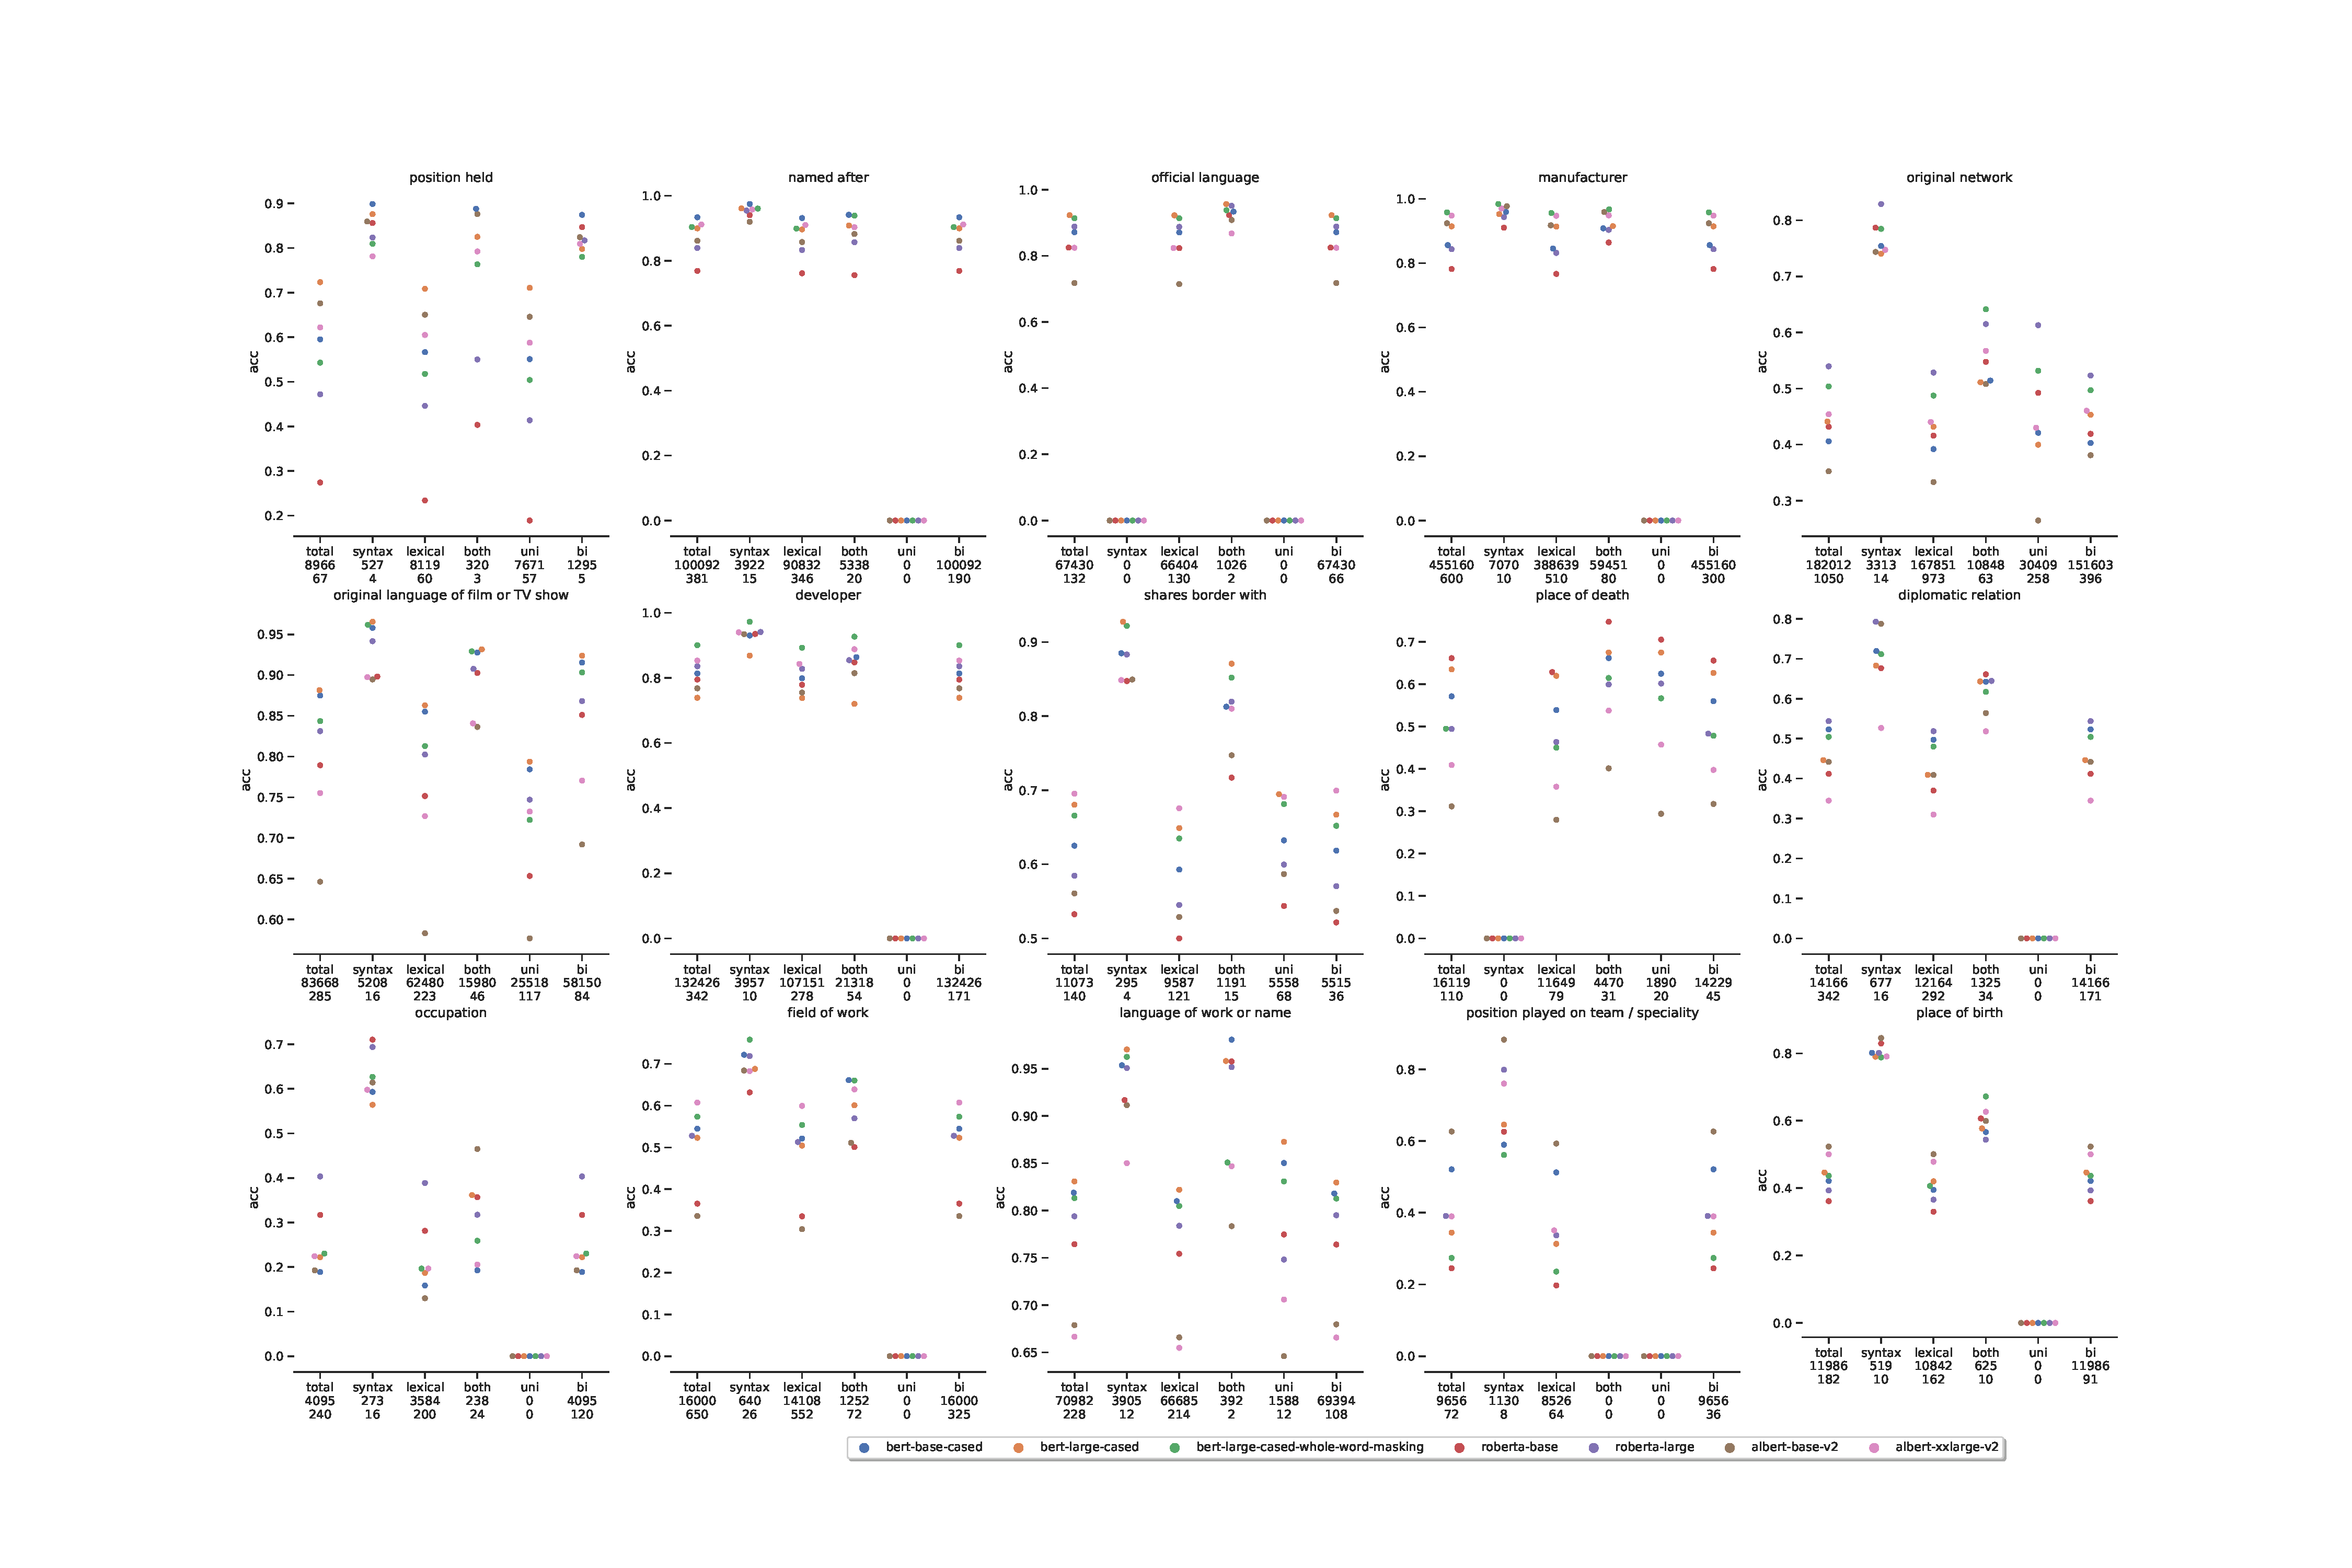
\includegraphics[width=1.\textwidth]{figures/results}

% \caption{Results summary, by relation, by split.}
% \label{fig:resuls}
% % \vspace{-6mm}
% \end{figure*}

% \begin{table*}[t]
% \small
    \centering
\resizebox{1\textwidth}{!}{%
\begin{tabular}{lrrrrrrrr}
\toprule
                              pattern &  know &  unk &  top@1 &  group-score &  const-subjs &  succ-patt &  succ-subjs &  consistency \\
\midrule
                             religion &                      0.35 &                        0.22 &      0.12 &            0.09 &                 0.09 &                  1.0 &                 0.88 &         0.34 \\
                       place of death &                      0.43 &                        0.32 &      0.42 &            0.04 &                 0.05 &                  1.0 &                 0.54 &         0.38 \\
                              capital &                      0.91 &                        0.40 &      0.70 &            0.57 &                 0.61 &                  1.0 &                 0.75 &         0.78 \\
                           instrument &                      0.48 &                        0.62 &      0.50 &            0.03 &                 0.05 &                  1.0 &                 0.85 &         0.50 \\
                             employer &                      0.38 &                        0.38 &      0.10 &            0.03 &                 0.11 &                  1.0 &                 0.27 &         0.38 \\
                headquarters location &                      0.65 &                        0.35 &      0.36 &            0.21 &                 0.25 &                  1.0 &                 0.53 &         0.51 \\
                        position held &                      0.49 &                        0.46 &      0.29 &            0.08 &                 0.11 &                  1.0 &                 0.65 &         0.48 \\
                            continent &                      0.92 &                        0.74 &      0.90 &            0.83 &                 0.85 &                  1.0 &                 0.97 &         0.91 \\
                            member of &                      0.92 &                        0.27 &      0.84 &            0.72 &                 0.74 &                  1.0 &                 0.89 &         0.85 \\
                              country &                      0.89 &                        0.74 &      0.60 &            0.54 &                 0.77 &                  1.0 &                 0.65 &         0.84 \\
                          subclass of &                      0.83 &                        0.53 &      0.61 &            0.56 &                 0.63 &                  1.0 &                 0.78 &         0.76 \\
                          instance of &                      0.51 &                        0.19 &      0.53 &            0.05 &                 0.05 &                  1.0 &                 0.86 &         0.47 \\
                              part of &                      0.62 &                        0.53 &      0.47 &            0.31 &                 0.57 &                  1.0 &                 0.51 &         0.57 \\
                             owned by &                      0.55 &                        0.23 &      0.51 &            0.21 &                 0.22 &                  1.0 &                 0.65 &         0.44 \\
                         record label &                      0.26 &                        0.28 &      0.06 &            0.00 &                 0.00 &                  1.0 &                 0.79 &         0.26 \\
                        field of work &                      0.28 &                        0.21 &      0.15 &            0.01 &                 0.01 &                  1.0 &                 0.39 &         0.23 \\
                        work location &                      0.74 &                        0.68 &      0.42 &            0.28 &                 0.42 &                  1.0 &                 0.59 &         0.72 \\
             language of work or name &                      0.70 &                        0.60 &      0.72 &            0.21 &                 0.23 &                  1.0 &                 0.85 &         0.69 \\
          twinned administrative body &                      0.57 &                        0.70 &      0.04 &            0.02 &                 0.37 &                  1.0 &                 0.07 &         0.69 \\
                         manufacturer &                      0.88 &                        0.33 &      0.90 &            0.62 &                 0.62 &                  1.0 &                 0.96 &         0.86 \\
                location of formation &                      0.59 &                        0.50 &      0.11 &            0.03 &                 0.13 &                  1.0 &                 0.18 &         0.52 \\
                                genre &                      0.52 &                        0.41 &      0.61 &            0.03 &                 0.03 &                  1.0 &                 0.79 &         0.49 \\
                    official language &                      0.87 &                        0.70 &      0.64 &            0.49 &                 0.64 &                  1.0 &                 0.81 &         0.84 \\
 position played on team / speciality &                      0.30 &                        0.32 &      0.06 &            0.00 &                 0.00 &                  1.0 &                 0.45 &         0.31 \\
                            developer &                      0.63 &                        0.28 &      0.71 &            0.22 &                 0.22 &                  1.0 &                 0.91 &         0.60 \\
                             location &                      0.56 &                        0.34 &      0.49 &            0.01 &                 0.01 &                  1.0 &                 0.70 &         0.49 \\
                          named after &                      0.78 &                        0.47 &      0.60 &            0.38 &                 0.41 &                  1.0 &                 0.80 &         0.71 \\
                    country of origin &                      0.67 &                        0.54 &      0.40 &            0.20 &                 0.25 &                  1.0 &                 0.63 &         0.62 \\
                     original network &                      0.29 &                        0.25 &      0.33 &            0.00 &                 0.00 &                  1.0 &                 0.82 &         0.28 \\
                       place of birth &                      0.46 &                        0.38 &      0.26 &            0.00 &                 0.01 &                  1.0 &                 0.32 &         0.41 \\
              applies to jurisdiction &                      0.94 &                        0.69 &      0.76 &            0.74 &                 0.82 &                  1.0 &                 0.83 &         0.90 \\
                           occupation &                      0.34 &                        0.35 &      0.01 &            0.00 &                 0.00 &                  1.0 &                 0.14 &         0.35 \\
                           capital of &                      0.95 &                        0.51 &      0.89 &            0.80 &                 0.82 &                  1.0 &                 0.92 &         0.92 \\
 original language of film or TV show &                      0.89 &                        0.90 &      0.58 &            0.50 &                 0.79 &                  1.0 &                 0.64 &         0.90 \\
               country of citizenship &                      0.74 &                        0.65 &      0.36 &            0.27 &                 0.32 &                  1.0 &                 0.68 &         0.71 \\
                   shares border with &                      0.54 &                        0.54 &      0.26 &            0.06 &                 0.14 &                  1.0 &                 0.54 &         0.54 \\
\bottomrule
\end{tabular}
}
    \caption{Additional results for the BERT-large model. }
    \label{tab:bert-results}
\end{table*}


\subsection{Consistency and Knowledge}

\yg{wdym by ``to asses the knowledge and ability of the different patterns to extract knowledge''? in particular, what is the first `knowledge'?}
To better understand the results, and assess the knowledge and ability of the different patterns to extract the correct knowledge of \resource{}, we report additional metrics that help to\am{remove "to"? unsure} understand the results. \sr{need a better motivation. e.g. ``In this section, we provide a finer-grained analysis, measuring consistency scores in various settings". But honestly this looks a bit like a checklist of different, unrelated experiments, and may be better pushed into an appendix.}

First, we report the percentage of triples that were predicted correctly by at least one of the patterns (Succ-Objs), and the percentage of patterns that successfully predicted the right object at least once (Succ-Patt). Succ-Objs quantifies the degree to which the knowledge is stored by the models, and Succ-Patt quantified the quality of the patterns to extract the knowledge.
Across models, all patterns successfully extracted the right
answer at least once, except for three models (bert-large and the two versions of albert) where one pattern in the `diplomatic relation'  did not succeed to classify any tuple.
On the other hand, some tuples are not predicted correctly by any of the patterns, as is shown in the Succ-Objs measure. Since most relations contain at least @@ patterns, we take it as evidence that this knowledge is not stored in the model. 
% \nk{This seems to suggest that it is the fault of the pattern that knowledge is not extracted from the model but an unsuccessful prediction across all models of the same tuple rather says that this knowledge is not stored} 
The average number of extractable tuples \am{extractable tuples?} is between 45.3\% to 63.0\%, depending on the model. Notably, the BERT based models are consistently better than the rest in extracting the knowledge. 

Next, we report LAMA results, that is\am{comma} the acc@1 accuracy\am{acc@1 accuracy is weird} of a model in predicting the object, using the original patterns from \citet{lama}. This metric inspects whether the first object within the candidate set of each relation is the correct answer. The reported numbers for this metric differ from \citet{lama} \am{reporting X\%} as we use a candidate set, as well as take only the KB triple where the objects are a single token in all models we inspect. The results range between 29.9 with albert-base to 45.6\am{should be \%?} with bert-large, being the best model in that aspect.
Additionally, we report another metric, which we call \textsc{Group-Score}, where a point is given only when all patterns predict the object correctly. This metric is much stricter than \textit{acc@1}, however, it provides a more robust metric, and better quantifies the degree to which the knowledge is encoded into the model. Overall, it combines both the requirement of a model to be consistent and correct. The results are much lower than the LAMA metric, as expected, but follow the same trend: albert-base perform worse, 17.0\% and bert-large performs best with 27.5\% accuracy.

\yg{give this part a paragraph title?}
Next, we measure the consistency results for the tuples
subset where at least one of the patterns for a specific
relation predicted the correct answer, as well as for the
subset where no pattern predicted the right answer correctly \am{correct answer, like previous line}
-- we refer to these metrics as \textsc{Know-Const} and \textsc{Unk-Const}, respectively.
A higher score on the first metric would suggest that storing the correct answer is related to the consistency of the model and performing consistent predictions across paraphrases.
Indeed, the results appear to support this claim. For instance, the Know-Const metric for bert-large is 62.4 and Unk-Const is 46.4. \nk{I would emphasize this even more and say that our graph is able to distinguish pattern dependent guessing and the other is knowledge stored in the model}
% point on a connection between acquiring the correct knowledge, and the ability to extract it robustly. 
% We refer to these metrics as \textsc{Know} and \textsc{Unk}, respectively, that stands for Knowledgeable and Unknowledgeable consistency.
The additional consistent measurement we report is Const-Objs, which measures the number of tuples that are predicted consistently across all patterns for a particular relation.
\ye{not sure if this one is important / alternatively maybe use this one instead of the main consistency score?}




% For brevity, we report the results solely on BERT-large, which achieved the highest results. The results can be viewed in Table \ref{tab:bert-results}.


An interesting observation from the results, is the clear superiority of the BERT models over the others, both in the factual knowledge correctness and consistency. This result, which we hypothesise to be due to the training data, may have a broader impact on the\am{remove the} models to come: Training bigger models on\am{with?} more data is not always beneficial. Since Wikipedia is likely the largest unified source of factual knowledge that exists in unstructured data,\yg{is it? maybe say ''a large''?} the focused\am{I don't like the word "focused"} training on it (besides from the book corpus) was likely to make the BERT models memorize\am{you never introduced memorization, just generalization} it better.
As such, models such as GPT-3 \cite{gpt3}, or other future models that solely train on more data with more parameters are not likely to be more consistent.\am{this is unsubstantiated, you can add "we hypothesize" to make this claim}% and retain more factual knowledge.


\subsection{Do PLMs Generalize Over Syntax?} 
% \sr{what does this title mean?}
Many papers found models (especially PLMs) to naturally encode syntax \cite{linzen2016assessing,marvin-linzen-2018-targeted,yoav-syntax,hewitt2019structural}. How does this reflect in their ability to abstract knowledge and produce it while controlling for syntactic variations?
We consider two scenarios: (1) the syntax is the only component that differs between the patterns and (2) both the syntax and the lexical choice remain the same.
Success on the first scenario indicates the ability of the model to abstract the knowledge, and extract it using different syntactic patterns. Success on the second indicates the abstraction over word order and tense. This way, we can test for consistency in models, while controlling for syntactic variation.\footnote{We consider two patterns to have the same syntax if the path between the entities are equal} 
% \sr{needs a footnote on our \emph{proxy} for syntactic change.}
% staying invariant to alternations while the syntax is the only component that differs, and when 
We parse all the patterns from \resource{} using a dependency parser \cite{spacy}\footnote{\url{https://spacy.io/}} and retain the path between the subject and object.
% Then, for every pattern pair, we split into two groups: (1) patterns where the only difference is the syntactic path, but the lexical items are equal, and (2) patterns where both the syntactic path and the lexical items are identical. \nk{This sentence seems repetitive}
% we filter out all cases where the syntactic path is different. 


The results are reported in Table \ref{}.  While the results are not comparable to the main results on the entire data, as they contain different patterns, overall the results are low: @@ for BERT-base, @@ for BERT-large, and @@ for ALBERT base. These results are surprising, since the ability to abstract over syntax is perhaps the easier abstraction, and was expected to perform better, given other results on PLMs syntactic abilities. \sr{not sure if we can say it's easier/harder.}

These results reminiscent of the findings of \citet{mccoy2019right}, which showed that models trained on an NLI dataset \cite{dagan-rte,snli} such as MNLI \cite{mnli}, are bound to use superficial syntactic heuristics, rather than more generalizable methods.
However, we demonstrate that even the\am{remove "the", use PLMs} pretrained models are susceptible to these errors. 

% \section{Experiments and Results}
\label{sec:experiments}


\begin{table*}[t]
% \small
    \centering
\resizebox{1\textwidth}{!}{%
\begin{tabular}{lllllllll}
\toprule
Models &       LAMA & Group-Score &    Succ-Pat &  Succ-Objs &  Know-Const &   Unk-Const &  Const-Objs & Consistency \\

\midrule
majority-baseline &  24.2+-20.7 &  24.2+-20.7 &  100.0+-0.0 &  24.9+-20.7 &  100.0+-0.0 &  100.0+-0.0 &  100.0+-0.0 &  100.0+-0.0 \\ \midrule
bert-base         &  44.1+-25.6 &  25.0+-25.5 &  100.0+-0.0 &  60.6+-23.5 &  61.4+-23.2 &  45.2+-20.6 &  32.5+-28.5 &  57.3+-22.3 \\
bert-large        &  45.6+-27.0 &  27.5+-27.6 &   99.7+-1.8 &  63.0+-25.2 &  62.4+-22.4 &  46.4+-18.5 &  34.2+-30.0 &  59.1+-21.5 \\
bert-large-wwm    &  45.4+-26.4 &  27.2+-27.6 &  100.0+-0.0 &  61.6+-23.2 &  62.6+-23.6 &  46.5+-18.7 &  33.8+-29.8 &  58.6+-22.7 \\ \midrule
roberta-base      &  36.7+-24.6 &  16.0+-19.8 &  100.0+-0.0 &  54.2+-24.5 &  53.3+-20.2 &  41.2+-15.3 &  21.7+-23.1 &  50.1+-18.4 \\
roberta-large     &  40.8+-26.1 &  21.3+-23.7 &  100.0+-0.0 &  58.5+-24.1 &  58.2+-21.1 &  44.4+-16.0 &  27.4+-25.6 &  54.8+-19.6 \\ \midrule
albert-base       &  29.9+-24.2 &  17.0+-22.2 &   99.7+-1.8 &  45.3+-25.7 &  56.1+-21.5 &  43.1+-18.0 &  25.1+-25.4 &  51.2+-19.8 \\
albert-xxlarge    &  39.5+-26.1 &  21.9+-25.7 &   99.7+-1.8 &  56.3+-25.8 &  56.7+-22.7 &  38.8+-14.7 &  26.8+-26.8 &  51.5+-21.1 \\
\bottomrule
\end{tabular}


}
    \caption{Consistency and knowledge results for the different models.}
    \label{tab:consistency_main}
\end{table*}

\subsection{Consistency}

The results for the different models are summarized in Table \ref{tab:consistency_main}.
% First, we report the average consistency results for all graphs, as describe in Section \ref{sec:eval}.
The last column (``Consistency'') shows the average results across all relations \yg{consider oredering the table columns in the order of their discussion}\am{I actually like it in the end, its easier to find in a glance}

The BERT-based models achieve higher scores over all the models\am{over the others, or the rest}. Moreover, there is a consistent improvement from the base to large\am{emph or quote 'base' and 'large'} versions of each model, although it is not always significantly \am{is there a significance test?} higher (e.g. 57.3\% to 59.1\% in BERT, and 50.1\% to 54.8\% in RoBERTa).
However, in contrast to many previous works that observed quantitative and qualitative improvements of RoBERTa-based models over BERT, in terms of consistency\am{comma} BERT is better than RoBERTa and ALBERT.\am{I would rephrase and say "BERT is more consistent than ...."}
Still, the overall results are remarkably low (59.1\% for the best model, \yg{meaning that out of XXX, YYY are ZZZ}), especially given the permissive evaluation that only looks at the candidate set.
We note that the results are highly variant between models and relations. For instance, the best performing model on the `capital of' relation achieves 94\%, whereas the best performing model on `owned by' is 44\%\am{is what? "achieves"?}. 
On the other hand, the models' performance on the `original language of film or TV show' relation, varies between 52\% and 90\% accuracy.
We report the full consistency results for each relation in the Appendix.

\begin{table}[t]
% \small
    \centering
\resizebox{1\columnwidth}{!}{%
\begin{tabular}{lrrr}
\toprule
Model&        Acc & Consistency & Consistent-Acc \\

\midrule
majority               &  23.1+-21.0 &  100.0+-0.0 &  23.1+-21.0 \\
\midrule
RoBERTa-med-small-1M &   11.2+-9.4 &  37.1+-11.0 &    2.8+-4.0 \\
\midrule
RoBERTa-base-10M     &  17.3+-15.8 &  29.8+-12.7 &    3.2+-5.1 \\
RoBERTa-base-100M    &  22.1+-17.1 &  31.5+-13.0 &    3.7+-5.3 \\
RoBERTa-base-1B      &  \textbf{38.0}+-23.4 &  \textbf{50.6}+-19.8 &  \textbf{18.0}+-16.0 \\
\bottomrule
\end{tabular}
}
    \caption{Knowledge and consistency results for the different RoBERTas, trained on increasing amounts of data. Best model for each metric is highlighted in bold.}
    \label{tab:robertas}
\end{table}

% \enote{hs}{below: i would prefer ``(training) corpus size''
%   over ``number of tokens'' if that's what you mean}

\paragraph{Effect of Pretraining Corpus Size}
Next, we study the question of whether the number of tokens used during the pretraining contributes to consistency.
We use the pretrained RoBERTas model provided by \citet{robertas} and repeat the experiments on four additional models.
These models are RoBERTa-based models, that were trained on a sample of Wikipedia and the book corpus, with varying training size, and parameters. In practice, we use one of the three published models for each configuration and report the average accuracy over the relations for each model in Table \ref{tab:robertas}.
Overall, the consistency and the knowledge scores (LAMA and Group-Score) improve when trained on more data. \nk{Maybe I missed it, did we say what the Group-Score is before?}\am{seems like not} However, there is an interesting outlier to this trend.
First, the model that was trained on one million tokens is more consistent than the models trained on ten and one-hundred million tokens. A potentially crucial difference is that this model is also smaller in terms of the number of parameters than the rest, in order to avoid overfitting. Still, it is nonetheless interesting that a model that is trained on significantly fewer\am{I would use "less"} data can achieve better consistency. On the other hand, the knowledge scores are lower, arguably due to less factual knowledge this model was exposed to during training.\am{due to the model being exposed to less factual knowledge during pretraining}

% Finally, the original RoBERTa that was trained on ten billion parameters, achieves the same consistency performance as the one trained on one billion tokens, suggesting a limit to the benefit of training examples in pretraining. \nk{not sure about this as the table is not there yet, but shouldn't it be: Finally, the original RoBERTa that was trained on ten billion tokens, achieves the same consistency performance as the one trained on one billion tokens, suggesting on a limit to the benefit of large training corpora. }



% \begin{table*}[t]
% \small
    \centering
\resizebox{1\textwidth}{!}{%
\begin{tabular}{lrrrrrrr}
\toprule
{} &  bert-base &  bert-large &  bert-large-wwm &  roberta-base &  roberta-large &  albert-base &  albert-xxlarge \\
\midrule
syn   &             0.50 &              0.53 &                                 0.53 &          0.44 &           0.48 &            0.44 &               0.45 \\
lex   &             0.56 &              0.59 &                                 0.58 &          0.51 &           0.54 &            0.52 &               0.49 \\
both  &             0.72 &              0.72 &                                 0.72 &          0.67 &           0.68 &            0.70 &               0.63 \\ \midrule
total &             0.52 &              0.54 &                                 0.54 &          0.45 &           0.50 &            0.46 &               0.46 \\
\bottomrule
\end{tabular}


}
    \caption{Consistent results aggregated on the different relations, by the different splits.}
    \label{tab:entailment-splits}
\end{table*}

% \begin{table*}[t]
% \small
    \centering
\resizebox{1\textwidth}{!}{%
\begin{tabular}{llrrrrrrr}
\toprule
     type & index &  bert-base-cased &  bert-large-cased &  bert-large-cased-wwm &  roberta-base &  roberta-large &  albert-base &  albert-xxlarge \\
\midrule
\multirow{3}{*}{consistency} & 1-1 &             0.76 &              0.82 &                                 0.84 &          0.58 &           0.73 &            0.66 &               0.80 \\
     & N-1 &             0.55 &              0.56 &                                 0.57 &          0.48 &           0.51 &            0.46 &               0.48 \\
     & N-M &             0.43 &              0.47 &                                 0.46 &          0.39 &           0.44 &            0.44 &               0.40 \\
\cline{1-9}
\multirow{3}{*}{syntactic} & 1-1 &             0.75 &              0.81 &                                 0.83 &          0.57 &           0.72 &            0.66 &               0.79 \\
     & N-1 &             0.53 &              0.55 &                                 0.56 &          0.46 &           0.49 &            0.44 &               0.47 \\
     & N-M &             0.41 &              0.45 &                                 0.44 &          0.38 &           0.43 &            0.42 &               0.40 \\
\cline{1-9}
\multirow{3}{*}{lexical} & 1-1 &             0.85 &              0.88 &                                 0.89 &          0.67 &           0.80 &            0.75 &               0.86 \\
     & N-1 &             0.59 &              0.60 &                                 0.62 &          0.55 &           0.57 &            0.51 &               0.51 \\
     & N-M &             0.45 &              0.53 &                                 0.48 &          0.40 &           0.44 &            0.52 &               0.39 \\
\cline{1-9}
\multirow{3}{*}{both} & 1-1 &             0.59 &              0.76 &                                 0.83 &          0.16 &           0.49 &            0.46 &               0.73 \\
     & N-1 &             0.75 &              0.76 &                                 0.74 &          0.69 &           0.72 &            0.72 &               0.69 \\
     & N-M &             0.68 &              0.66 &                                 0.68 &          0.64 &           0.64 &            0.68 &               0.54 \\
\bottomrule
\end{tabular}

}
    \caption{Consistent results aggregated on the different relations, by the different splits.}
    \label{tab:entailment-splits}
\end{table*}


% \begin{figure*}[t!]
% \centering

% 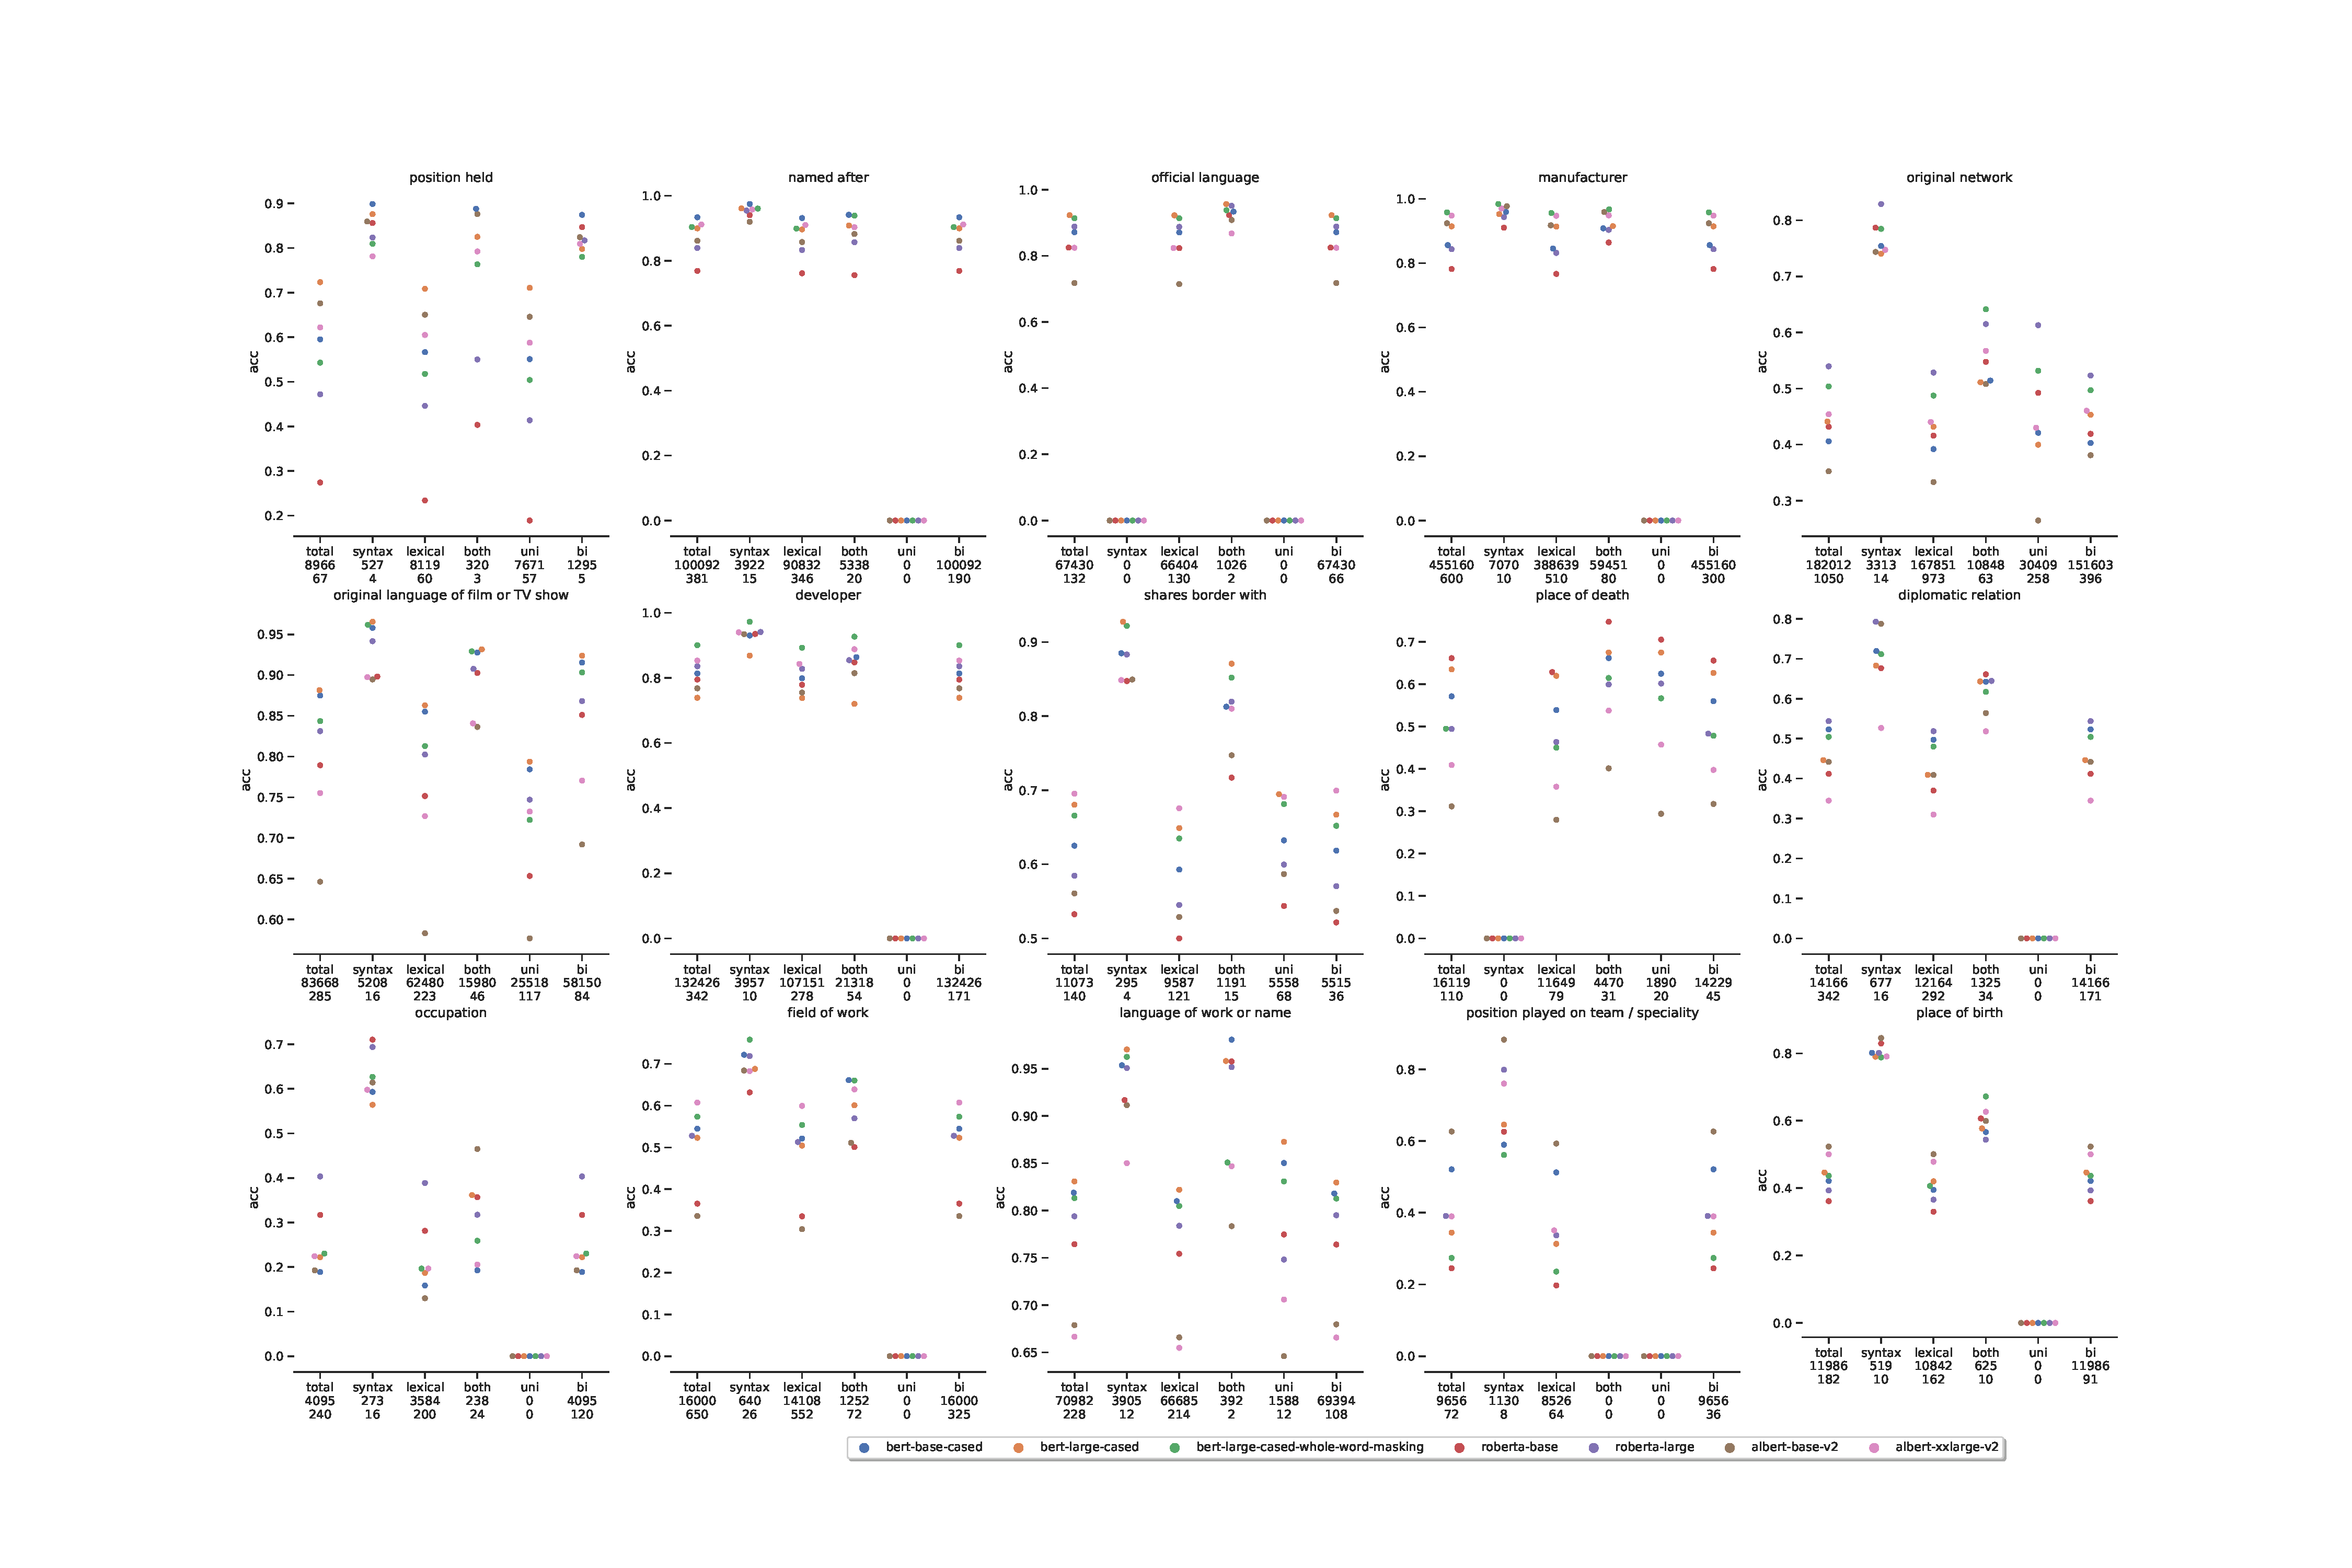
\includegraphics[width=1.\textwidth]{figures/results}

% \caption{Results summary, by relation, by split.}
% \label{fig:resuls}
% % \vspace{-6mm}
% \end{figure*}

% \begin{table*}[t]
% \small
    \centering
\resizebox{1\textwidth}{!}{%
\begin{tabular}{lrrrrrrrr}
\toprule
                              pattern &  know &  unk &  top@1 &  group-score &  const-subjs &  succ-patt &  succ-subjs &  consistency \\
\midrule
                             religion &                      0.35 &                        0.22 &      0.12 &            0.09 &                 0.09 &                  1.0 &                 0.88 &         0.34 \\
                       place of death &                      0.43 &                        0.32 &      0.42 &            0.04 &                 0.05 &                  1.0 &                 0.54 &         0.38 \\
                              capital &                      0.91 &                        0.40 &      0.70 &            0.57 &                 0.61 &                  1.0 &                 0.75 &         0.78 \\
                           instrument &                      0.48 &                        0.62 &      0.50 &            0.03 &                 0.05 &                  1.0 &                 0.85 &         0.50 \\
                             employer &                      0.38 &                        0.38 &      0.10 &            0.03 &                 0.11 &                  1.0 &                 0.27 &         0.38 \\
                headquarters location &                      0.65 &                        0.35 &      0.36 &            0.21 &                 0.25 &                  1.0 &                 0.53 &         0.51 \\
                        position held &                      0.49 &                        0.46 &      0.29 &            0.08 &                 0.11 &                  1.0 &                 0.65 &         0.48 \\
                            continent &                      0.92 &                        0.74 &      0.90 &            0.83 &                 0.85 &                  1.0 &                 0.97 &         0.91 \\
                            member of &                      0.92 &                        0.27 &      0.84 &            0.72 &                 0.74 &                  1.0 &                 0.89 &         0.85 \\
                              country &                      0.89 &                        0.74 &      0.60 &            0.54 &                 0.77 &                  1.0 &                 0.65 &         0.84 \\
                          subclass of &                      0.83 &                        0.53 &      0.61 &            0.56 &                 0.63 &                  1.0 &                 0.78 &         0.76 \\
                          instance of &                      0.51 &                        0.19 &      0.53 &            0.05 &                 0.05 &                  1.0 &                 0.86 &         0.47 \\
                              part of &                      0.62 &                        0.53 &      0.47 &            0.31 &                 0.57 &                  1.0 &                 0.51 &         0.57 \\
                             owned by &                      0.55 &                        0.23 &      0.51 &            0.21 &                 0.22 &                  1.0 &                 0.65 &         0.44 \\
                         record label &                      0.26 &                        0.28 &      0.06 &            0.00 &                 0.00 &                  1.0 &                 0.79 &         0.26 \\
                        field of work &                      0.28 &                        0.21 &      0.15 &            0.01 &                 0.01 &                  1.0 &                 0.39 &         0.23 \\
                        work location &                      0.74 &                        0.68 &      0.42 &            0.28 &                 0.42 &                  1.0 &                 0.59 &         0.72 \\
             language of work or name &                      0.70 &                        0.60 &      0.72 &            0.21 &                 0.23 &                  1.0 &                 0.85 &         0.69 \\
          twinned administrative body &                      0.57 &                        0.70 &      0.04 &            0.02 &                 0.37 &                  1.0 &                 0.07 &         0.69 \\
                         manufacturer &                      0.88 &                        0.33 &      0.90 &            0.62 &                 0.62 &                  1.0 &                 0.96 &         0.86 \\
                location of formation &                      0.59 &                        0.50 &      0.11 &            0.03 &                 0.13 &                  1.0 &                 0.18 &         0.52 \\
                                genre &                      0.52 &                        0.41 &      0.61 &            0.03 &                 0.03 &                  1.0 &                 0.79 &         0.49 \\
                    official language &                      0.87 &                        0.70 &      0.64 &            0.49 &                 0.64 &                  1.0 &                 0.81 &         0.84 \\
 position played on team / speciality &                      0.30 &                        0.32 &      0.06 &            0.00 &                 0.00 &                  1.0 &                 0.45 &         0.31 \\
                            developer &                      0.63 &                        0.28 &      0.71 &            0.22 &                 0.22 &                  1.0 &                 0.91 &         0.60 \\
                             location &                      0.56 &                        0.34 &      0.49 &            0.01 &                 0.01 &                  1.0 &                 0.70 &         0.49 \\
                          named after &                      0.78 &                        0.47 &      0.60 &            0.38 &                 0.41 &                  1.0 &                 0.80 &         0.71 \\
                    country of origin &                      0.67 &                        0.54 &      0.40 &            0.20 &                 0.25 &                  1.0 &                 0.63 &         0.62 \\
                     original network &                      0.29 &                        0.25 &      0.33 &            0.00 &                 0.00 &                  1.0 &                 0.82 &         0.28 \\
                       place of birth &                      0.46 &                        0.38 &      0.26 &            0.00 &                 0.01 &                  1.0 &                 0.32 &         0.41 \\
              applies to jurisdiction &                      0.94 &                        0.69 &      0.76 &            0.74 &                 0.82 &                  1.0 &                 0.83 &         0.90 \\
                           occupation &                      0.34 &                        0.35 &      0.01 &            0.00 &                 0.00 &                  1.0 &                 0.14 &         0.35 \\
                           capital of &                      0.95 &                        0.51 &      0.89 &            0.80 &                 0.82 &                  1.0 &                 0.92 &         0.92 \\
 original language of film or TV show &                      0.89 &                        0.90 &      0.58 &            0.50 &                 0.79 &                  1.0 &                 0.64 &         0.90 \\
               country of citizenship &                      0.74 &                        0.65 &      0.36 &            0.27 &                 0.32 &                  1.0 &                 0.68 &         0.71 \\
                   shares border with &                      0.54 &                        0.54 &      0.26 &            0.06 &                 0.14 &                  1.0 &                 0.54 &         0.54 \\
\bottomrule
\end{tabular}
}
    \caption{Additional results for the BERT-large model. }
    \label{tab:bert-results}
\end{table*}


\subsection{Consistency and Knowledge}

\yg{wdym by ``to asses the knowledge and ability of the different patterns to extract knowledge''? in particular, what is the first `knowledge'?}
To better understand the results, and assess the knowledge and ability of the different patterns to extract the correct knowledge of \resource{}, we report additional metrics that help to\am{remove "to"? unsure} understand the results. \sr{need a better motivation. e.g. ``In this section, we provide a finer-grained analysis, measuring consistency scores in various settings". But honestly this looks a bit like a checklist of different, unrelated experiments, and may be better pushed into an appendix.}

First, we report the percentage of triples that were predicted correctly by at least one of the patterns (Succ-Objs), and the percentage of patterns that successfully predicted the right object at least once (Succ-Patt). Succ-Objs quantifies the degree to which the knowledge is stored by the models, and Succ-Patt quantified the quality of the patterns to extract the knowledge.
Across models, all patterns successfully extracted the right
answer at least once, except for three models (bert-large and the two versions of albert) where one pattern in the `diplomatic relation'  did not succeed to classify any tuple.
On the other hand, some tuples are not predicted correctly by any of the patterns, as is shown in the Succ-Objs measure. Since most relations contain at least @@ patterns, we take it as evidence that this knowledge is not stored in the model. 
% \nk{This seems to suggest that it is the fault of the pattern that knowledge is not extracted from the model but an unsuccessful prediction across all models of the same tuple rather says that this knowledge is not stored} 
The average number of extractable tuples \am{extractable tuples?} is between 45.3\% to 63.0\%, depending on the model. Notably, the BERT based models are consistently better than the rest in extracting the knowledge. 

Next, we report LAMA results, that is\am{comma} the acc@1 accuracy\am{acc@1 accuracy is weird} of a model in predicting the object, using the original patterns from \citet{lama}. This metric inspects whether the first object within the candidate set of each relation is the correct answer. The reported numbers for this metric differ from \citet{lama} \am{reporting X\%} as we use a candidate set, as well as take only the KB triple where the objects are a single token in all models we inspect. The results range between 29.9 with albert-base to 45.6\am{should be \%?} with bert-large, being the best model in that aspect.
Additionally, we report another metric, which we call \textsc{Group-Score}, where a point is given only when all patterns predict the object correctly. This metric is much stricter than \textit{acc@1}, however, it provides a more robust metric, and better quantifies the degree to which the knowledge is encoded into the model. Overall, it combines both the requirement of a model to be consistent and correct. The results are much lower than the LAMA metric, as expected, but follow the same trend: albert-base perform worse, 17.0\% and bert-large performs best with 27.5\% accuracy.

\yg{give this part a paragraph title?}
Next, we measure the consistency results for the tuples
subset where at least one of the patterns for a specific
relation predicted the correct answer, as well as for the
subset where no pattern predicted the right answer correctly \am{correct answer, like previous line}
-- we refer to these metrics as \textsc{Know-Const} and \textsc{Unk-Const}, respectively.
A higher score on the first metric would suggest that storing the correct answer is related to the consistency of the model and performing consistent predictions across paraphrases.
Indeed, the results appear to support this claim. For instance, the Know-Const metric for bert-large is 62.4 and Unk-Const is 46.4. \nk{I would emphasize this even more and say that our graph is able to distinguish pattern dependent guessing and the other is knowledge stored in the model}
% point on a connection between acquiring the correct knowledge, and the ability to extract it robustly. 
% We refer to these metrics as \textsc{Know} and \textsc{Unk}, respectively, that stands for Knowledgeable and Unknowledgeable consistency.
The additional consistent measurement we report is Const-Objs, which measures the number of tuples that are predicted consistently across all patterns for a particular relation.
\ye{not sure if this one is important / alternatively maybe use this one instead of the main consistency score?}




% For brevity, we report the results solely on BERT-large, which achieved the highest results. The results can be viewed in Table \ref{tab:bert-results}.


An interesting observation from the results, is the clear superiority of the BERT models over the others, both in the factual knowledge correctness and consistency. This result, which we hypothesise to be due to the training data, may have a broader impact on the\am{remove the} models to come: Training bigger models on\am{with?} more data is not always beneficial. Since Wikipedia is likely the largest unified source of factual knowledge that exists in unstructured data,\yg{is it? maybe say ''a large''?} the focused\am{I don't like the word "focused"} training on it (besides from the book corpus) was likely to make the BERT models memorize\am{you never introduced memorization, just generalization} it better.
As such, models such as GPT-3 \cite{gpt3}, or other future models that solely train on more data with more parameters are not likely to be more consistent.\am{this is unsubstantiated, you can add "we hypothesize" to make this claim}% and retain more factual knowledge.


\subsection{Do PLMs Generalize Over Syntax?} 
% \sr{what does this title mean?}
Many papers found models (especially PLMs) to naturally encode syntax \cite{linzen2016assessing,marvin-linzen-2018-targeted,yoav-syntax,hewitt2019structural}. How does this reflect in their ability to abstract knowledge and produce it while controlling for syntactic variations?
We consider two scenarios: (1) the syntax is the only component that differs between the patterns and (2) both the syntax and the lexical choice remain the same.
Success on the first scenario indicates the ability of the model to abstract the knowledge, and extract it using different syntactic patterns. Success on the second indicates the abstraction over word order and tense. This way, we can test for consistency in models, while controlling for syntactic variation.\footnote{We consider two patterns to have the same syntax if the path between the entities are equal} 
% \sr{needs a footnote on our \emph{proxy} for syntactic change.}
% staying invariant to alternations while the syntax is the only component that differs, and when 
We parse all the patterns from \resource{} using a dependency parser \cite{spacy}\footnote{\url{https://spacy.io/}} and retain the path between the subject and object.
% Then, for every pattern pair, we split into two groups: (1) patterns where the only difference is the syntactic path, but the lexical items are equal, and (2) patterns where both the syntactic path and the lexical items are identical. \nk{This sentence seems repetitive}
% we filter out all cases where the syntactic path is different. 


The results are reported in Table \ref{}.  While the results are not comparable to the main results on the entire data, as they contain different patterns, overall the results are low: @@ for BERT-base, @@ for BERT-large, and @@ for ALBERT base. These results are surprising, since the ability to abstract over syntax is perhaps the easier abstraction, and was expected to perform better, given other results on PLMs syntactic abilities. \sr{not sure if we can say it's easier/harder.}

These results reminiscent of the findings of \citet{mccoy2019right}, which showed that models trained on an NLI dataset \cite{dagan-rte,snli} such as MNLI \cite{mnli}, are bound to use superficial syntactic heuristics, rather than more generalizable methods.
However, we demonstrate that even the\am{remove "the", use PLMs} pretrained models are susceptible to these errors. 

\section{Analysis}
\label{sec:analysis}


\begin{table*}[t]
% \small
    \centering
\resizebox{1\textwidth}{!}{%
\begin{tabular}{llllllll}
\toprule
Subject & Object & Pattern \#1 & Pattern \#2 & Pattern \#3 & Pred \#1 & Pred \#2 & Pred \#3 \\
\midrule

% Adam Kendon & London & [X] was born in [Y]. & [X] is originally from [Y]. & The country of origin of [X] is [Y]. & \hltrue{London} & \hltrue{London} & \hlfalseo{Ireland} \\
Adriaan Pauw & Amsterdam & [X] was born in [Y]. & [X] is native to [Y]. & [X] is a [Y]-born person. & \hltrue{Amsterdam} & \hlfalseo{Madagascar} & \hlfalset{Luxembourg} \\
Nissan Livina Geniss & Nissan & [X] is produced by [Y]. & [X] is created by [Y]. & [X], created by [Y]. & \hltrue{Nissan} & \hlfalseo{Renault} & \hlfalseo{Renault} \\
Arab League & Asia & [X] belongs to the continent of [Y]. & [X] is located in [Y]. &  [X] is a part of the continent of [Y]. & \hltrue{Asia} & \hlfalseo{Europe} & \hlfalset{Africa} \\ 
% Albania & Serbia & [X] shares border with [Y]. & [Y] borders with [X]. & [Y] shares the border with [X] & \hlfalseo{Greece} & \hlfalset{Turkey} & \hlfalsetr{Kosovo} \\
iCloud & Apple & [X] is developed by [Y]. & [X], created by [Y]. & [X] was created by [Y] & \hlfalseo{Microsoft} & \hlfalset{Google} & \hlfalsetr{Sony} \\
\midrule

Yahoo! Messenger & Yahoo & [X], a product created by [Y] & [X], a product developed by [Y] & [Y], that developed [X] & \hlfalseo{Microsoft} & \hlfalseo{Microsoft} & \hlfalseo{Microsoft} \\
Wales & Cardiff & The capital of [X] is [Y] . & [X]'s capital, [Y]. & [X]'s capital city, [Y]. & \hltrue{Cardiff} & \hltrue{Cardiff} & \hltrue{Cardiff} \\

\bottomrule
\end{tabular}


}
    \caption{Predictions of BERT-large-cased. Presenting the
      subjects and objects taken from T-REx \cite{trex}, as
      well as three different patterns from our resource and
      their predictions. The predictions are colored in blue
      if the model predicted correctly (out of the candidate
      list), and in red otherwise. If there is more than a
      single erroneous prediction, it is colored by a different red.}
    \label{tab:predictions}
\end{table*}



\subsection{Qualitative Analysis}
To better understand the factors affecting consistent
predictions, we inspect the predictions of BERT-large on the
patterns shown  in Table \ref{tab:predictions}.
We highlight several cases:
The predictions in Example \#1 are inconsistent, and correct for the first pattern (\textit{Amsterdam}), but not for the other two (\textit{Madagascar} and \textit{Luxembourg}). 
The predictions in Example \#2 also show a single pattern that predicted the right object; however, the two other patterns, which are lexically similar, predicted the same, wrong answer -- \textit{Renault}.
% However, the third pattern prediction is related in the sense that Ireland is close to London. \ye{is the Ireland-London argument convincing?}
Next, the patterns of Example \#3
produced two factually correct answers out of three (\textit{Greece}, \textit{Kosovo}), but simply do not correspond to the gold
object in T-REx (\textit{Albania}), since this is an M-N relation. Note that this relation is not part of the consistency evaluation, but the determinism evaluation.
The three different predictions in example \#4 are all incorrect.
% The last row of the upper part demonstrates three different predictions, all factually incorrect. 
% Note that even when more than a single answer is correct, we still argue that the model should make consistent predictions.
Finally, the two last predictions demonstrate consistent predictions:
Example \#5 is consistent but factually incorrect (even though the correct answer is a substring of the subject), and finally, Example \#6
is consistent and factual.
% fact the object is a substring of the subject).





\begin{figure}[t!]
\centering
% \vspace{-0.1in}
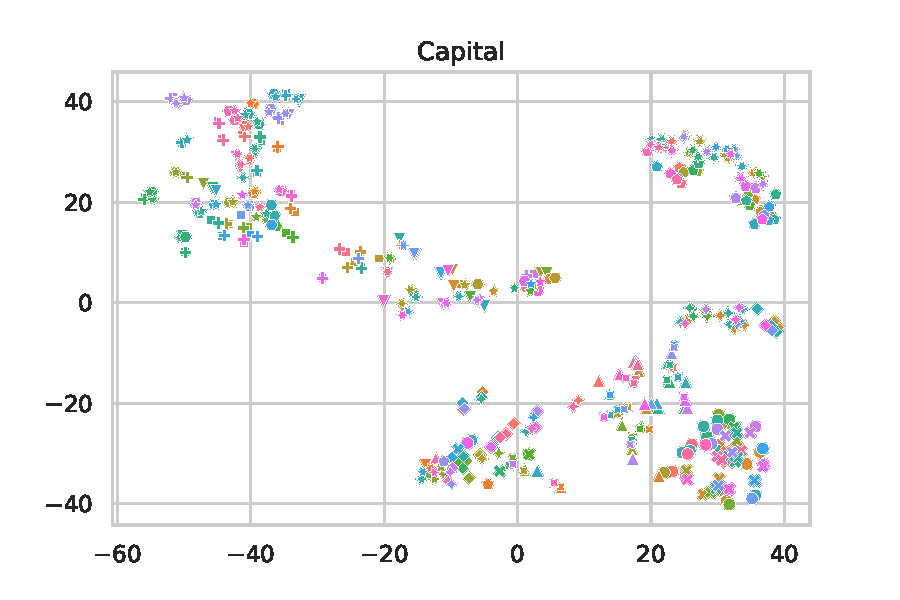
\includegraphics[width=1\columnwidth]{figures/capital-bert-large}


\caption{t-SNE of the encoded patterns from the
  \textit{capital} relation. The colors
  represent the different subjects, while the shapes
  represent patterns. A knowledge-focused representation
  should cluster based on identical subjects (color), but
  instead the clustering is according to identical patterns (shape).}
%   \vspace{-0.2in}
\label{fig:tsne-emb}

\end{figure}

\subsection{Representation Analysis}


To provide insights on the models' representations, we inspect these after encoding the patterns.

Motivated by previous work that found that words with the same syntactic structure cluster together \cite{chi-etal-2020-finding,ravfogel-etal-2020-unsupervised} we perform a similar experiment to test if this behavior replicates with respect to knowledge:
We encode the patterns, after filling the placeholders with subjects and masked tokens and inspect the last layer representations in the masked token position.
When plotting the results using t-SNE \cite{tsne} we mainly
observe clustering based on the patterns, which suggests
that encoding of knowledge of the entity is not the main component of the representations.
Figure \ref{fig:tsne-emb} demonstrates
this for BERT-large encodings of the \textit{capital} relation, which is highly consistent.\footnote{While some patterns are clustered based on the subjects (upper-left part), most of them are clustered based on patterns.}
To provide a more quantitative assessment of this phenomenon, 
we also cluster the representations and set the number of centroids based on:\footnote{Using the KMeans algorithm.} (1) the number of patterns in each relation, which aims to capture pattern-based clusters, and (2) the number of subjects in each relation, which aims to capture entity-based clusters. This would allow for a perfect clustering, in the case of perfect alignment between the representation and the inspected property.
We measure the purity of these clusters using V-measure and observe that the clusters are mostly grouped by the patterns, rather than the subjects.
% Finally, we compute the correlation between the distance of two representations, and whether their predictions are consistent. 
Finally, we compute the spearman correlation between the consistency scores and the V-measure of the representations.
However, the correlation between these variables is close to zero,\footnote{Except for BERT-large whole-word-masking, where the correlation is 39.5 ($p<0.05$).} therefore not explaining the models' behavior.
We repeated these experiments while inspecting the objects instead of the subjects, and found similar trends.
This finding is interesting since it means that (1) these representations are not knowledge-focused, i.e., their main component does not relate to knowledge, and (2) the representation by its entirety does not explain the behavior of the model, and thus only a subset of the representation does. %\nk{What do you mean by saying: only a subset of the representation does?} 
This finding is consistent with previous work that observed similar trends for linguistic tasks \cite{amnesic_probing}.
We hypothesize that this disparity between the
representation and the behavior of the model may be explained by a situation where the distance between representations largely does not reflect the distance between predictions, but rather other, behaviorally irrelevant factors of a sentence.
% We believe that the explanation of these findings is that the relevant information for the word prediction, lies in a subspace of the original representation, and thus much of the encoded information is in practice not relevant for the prediction. \sr{I don't understand this explanation. I'd write something like ``We hypothesize that this disparity between representation and behavior may be explained by a situation where distances between representations largely do not reflect the distance between predictions, but rather reflect other, behaviorally-irrelevant factors of each sentence"}.


% We encode the patterns, populated with 50 random subjects along with the masked token, and inspect the final layer in the masked token index for all the paraphrases of multiple relations.
% Then, we use t-SNE \cite{tsne} and present the results in Figure \ref{fig:tsne-emb} in the appendix.
% Each point represents a specific tuple and is colored by the subjects, and the shape stands for the pattern.
% A good representation would cluster the vectors together based on the subject, as then the predictions would more likely to be consistent. However, clusters based on patterns would suggest a worse encoding, since the subjects, which are of great importance in these paraphrases, are less taken into account in the representation.

% We display the t-SNE figures for two relations, \textit{Language  of work or name} and \textit{Capital} in Figure \ref{fig:tsne-emb}.
% It is clear that the first figure clusters mainly on the patterns, whereas the second figure clusters mainly on the subjects. These results are also consistent with the performance of these relations: @@\% and @@\%, which suggests a better representation for the latter.
% Additionally, we also perform clustering for the representations,\footnote{Using the KMeans algorithm.} once with the number of subjects and once with the number patterns, given as an oracle, hoping to fit the subjects or patterns clusters. Then, we calculate the v-measure metric for measuring the purity of each cluster.
% A higher score on the subject-based would suggest a representation that better fits the purpose of a KB.
% The v-measure results for these patterns are presented in Table \ref{tab:vmeasure-small}.
% As expected, the pattern-based clustering is better for the \textit{language of work or name} relation is higher than the subject-based, and vice versa for the \textit{capital} relation.
% The full clustering measures for all relations are reported in the Appendix.

% \begin{table}[t]
% \small
    \centering
% \resizebox{1\textwidth}{!}{%
\begin{tabular}{lrr}
\toprule
                                          Pattern &  pattern &  subject \\
\midrule
     language of work or name &            0.72 &            0.24 \\
                      capital &            0.41 &            0.62 \\
\bottomrule
\end{tabular}

% }
    \caption{V-measure clustering performance for the two relations. Reporting the results for clustering based on the pattern, and based on the subjects.}
    \label{tab:vmeasure-small}
\end{table}




\section{Improving Consistency in PLMs}
\label{sec:adding_consistency}

In the previous sections, we showed pretrained models are generally not consistent in their predictions, and previous works have noticed the lack of this property in a variety of downstream tasks.
% , and since PLMs are used for downstream tasks, lack of consistency is likely to affect them as well. 
% \nk{suggestion: cut: "lack of consistency is likely to affect them as well." , add: 
An ideal model would exhibit the consistency property after pretrained, and will then be able to transfer it to different downstream tasks. We therefor ask:
% Ideally, a consistent PLM would also reflect this property in downstream tasks.
Can we enhance current PLMs and make them more consistent?

\subsection{Consistency Improved PLM}
% \nk{Maybe we need to emphasize already when introducing this that this is more of a case study rather than solving the issue}
We propose a method to improve the consistency of PLMs, by continuing the pretaining step, with a novel consistency loss. %\nk{Should we refer to the paper that does it in a similar way?}
We make use of the TREx triples and the paraphrases from \resource{}.

Given a relation $r_i$, we
assume we have a set of $k$ paraphrased patterns for $R_i$,
$P_i=\{P_1^i, P_2^i, \dots, P_k^i\}$.
%, each $P_j^i$ represents a paraphrase of some relation $R^i$.
We use a PLM to encode all patterns in $P_i$, after populating a subject and a mask token that corresponds to the relation $r_i$. Finally we expect the model to make the same prediction for the masked token.
% Then we consider the probability distribution over the vocabulary of the masked word, denoted by $D^i_l$. Our goal is to make the distribution of every pair $D^i_l,D^i_m$ as close as possible.


\paragraph{Consistency Loss Function}
% Given two paraphrases from \resource{}, we expect the predictions of the masked tokens to be identical. However, as we showed in the previous sections, it is not the case. \nk{this is repeating the intro of section 8}
As we evaluate the model using the top-1 prediction, a possible consistency loss would require these predictions to be identical:
\begin{gather*} 
\min_{\theta} sim(\argmax Q_m, \argmax Q_n)\\
s.t. Q_n = f(P_n; \theta), Q_m = f(P_m; \theta)
\end{gather*}
where $Q_n,Q_m$ are the distribution over the vocabulary for a pattern $P_n,P_m$ respectively, and $f$ is the encoding function, e.g. BERT, with parameters $\theta$.


However, this is a hard constraint and is hard to learn, due to the discrete and non-differential nature of the argmax, therefore we use a softer constraint instead.
Instead of optimizing for the same argmax, we optimize for the same distribution.
% We propose to enforce consistency, by requiring the distribution of the masked tokens to be identical. 
We use KL Divergence (DKL) to approach these distributions $Q$. Since DKL is not a symmetric metric, we use DKL to function on both sides for two patterns $P^i_m,P^i_n$:
$D_{KL}(Q^i_n||Q^i_m) + D_{KL} (Q^i_m||Q^i_n)$

As most of the vocabulary is not relevant for the
predictions, in practice we filter it down to the candidate set, of each relation \ref{sec:framework}. Moreover, since we are motivated by maintaining the original capabilities of the model, focusing on the candidate set helps to achieve this goal since most of the vocabulary is not affected by our new loss.
From preliminary results, we noticed that using only the candidate set is beneficial.

In practice, as we typically have multiple paraphrases, we use all of them, which can help in enforcing a more general solution. Thus, the consistency loss consist of all possible patterns pairs, for a particular relation $R^i$ would be:
\[
\mathcal{L}_{c} = \sum_{n=1}^k \sum_{m=n+1}^k D_{KL}(Q^i_m||Q^i_n) + D_{KL}(Q^i_n||Q^i_m)
\]


\paragraph{MLM Loss}
Since the consistency loss is different from the original Cross-Entropy loss the MLM was trained on, we find it important to continue the MLM loss on text data, as was observed in previous work \cite{geva2020injecting}.

We consider two alternatives for continuing the pretraining objective: (1) MLM on Wikipedia and (2) MLM on the patterns of the relations used for the consistency loss. In practice, we find that the latter works better. We denote this loss by $\mathcal{L}_{MLM}$


\paragraph{Consistency Guided MLM Continual Training}

Combining the novel consistency loss introduced above, with the regular MLM loss, we continue the PLM training by combining the two losses. The combination of the two losses is determined by a hyperparameter $\lambda$, to make the following final loss function:

\[
\mathcal{L} = \lambda \mathcal{L}_c + \mathcal{L}_{MLM}
\]

The above loss is computed per relation, for one KB tuple $d_j^i$. In practice, we have many of these instances, which we require to behave similarly. Therefore, we batch together $n$ tuples from the same relation and apply the same loss function to all of them.


\subsection{Setup}

% \paragraph{Relations used for training}
% The TREx relations contain different types and contain many location-related relations. 
Since we evaluate our method on relations other than the ones we train on, it's better to avoid relations of the same type (e.g. location-based relations, which are very common in TREx).
Moreover, our method is aimed to be simple, effective, and requires only minimal supervision, therefore we opt to use only a minimal number of relations for training.
In practice, we use only three relations: \textit{original-language}, \textit{named-after}, and \textit{original-network} that were chosen randomly, out of the non-location related relations.\footnote{Since many of the relations in t-REX are location-based we wish to avoid a train-test leakage.} % \nk{People would not understand why we exclude locations. I would cut this?}.
Since we train only on three relations, and the paraphrases are short, we manage to include many tuples in each batch, resulting in a short training phase.
For validation, we randomly pick three relations of the remaining relations and use the remaining twenty-five for testing.

We perform minimal tuning of the parameters, to pick the best model, train for 3 epochs, and select the best model based on the group score on the validation set.
For efficiency reasons, we use the base version of BERT but expect other models to behave similarly.


\subsection{Improved Consistency Results}

\begin{table}[t]
% \small
    \centering
\resizebox{1\columnwidth}{!}{%
\begin{tabular}{lrrr}
\toprule
Model &        Accuracy & Consistency & Consistent-Acc \\
\midrule


majority   &  24.4+-22.5 &  100.0+-0.0 &  24.4+-22.5 \\
\midrule
BERT-base  &  45.6+-27.6 &  58.2+-23.9 &  27.3+-24.8 \\
BERT-ft    &  \textbf{\textul{47.4}}+-27.3 &  \textbf{64.0}+-22.9 &  \textbf{\textul{33.2}}+-27.0 \\
\quad -consistency &  46.9+-27.6 &  60.9+-22.6 &  30.9+-26.3 \\
\quad -typed     &  46.5+-27.1 &  62.0+-21.2 &  31.1+-25.2 \\
\quad -MLM       &  16.9+-21.1 &  \textul{80.8}+-27.1 &   9.1+-11.5 \\

\bottomrule
\end{tabular}

}

    \caption{Knowledge and consistency results for the baseline, BERT base, and our model. 
    % We report the \textit{Accuracy} using the original patterns from LAMA, the \textit{Consistency}, and \textit{Consistency-Acc} metrics. 
    The results are average over the 25 test relations. Bolded numbers signifies best performance between the baseline and the finetuned model, underline signifies the best performance including the ablations.}
    \label{tab:consistency-ft}
    
    \vspace{-0.2in}
\end{table}

The results are presented in Table \ref{tab:consistency-ft}. We report the aggregated results for all of the relations, apart from those that were used for training or validation. As in the previous section, we report the mean over the inspected relations and the standard deviation.
We report the results of the majority baseline (first row), as well as the vanilla BERT-base model that we then fine-tune on (second row). Finally, we report the results of our new model (third row).
First, we note the significant improvement in consistency with our model: from 58.2\% in BERT-base to 64.0\% in our model, an increase of 5.8 points.
% \nk{I would emphasize here again that it was able to transfer consistency from the seen to the unseen relations and we should maybe add that this in not only syntax based (is it?)}
The LAMA score, also improves from the BERT baseline, from 45.6\% to 47.4\%. Finally, and most importantly, we see an increase of 5.9 points to the Group-Score, which is achieved due to the improved consistency of the model.
Notably, these improvements arises from training on merely three relations, meaning that the model improved its consistency ability and generalized to new relations.
We also measure the statistical significance of our method compared to the BERT baseline, using McNemar's test (following \citet{dror2018hitchhiker,dror2020statistical}) and find all results to be significant ($p<<0.01$)

We also perform an ablation study to quantify the utility of the different components. First, report on the finetuned model without the consistency loss (-consistency). Interestingly, it does improve over the baseline (BERT-base), but it lag behind our full model.
Second, applying our loss on the candidate set rather than on the entire vocabulary is beneficial (-typed). Finally, by not performing the MLM training on the generated patterns (-MLM), the consistency results improved significantly (80.8), however, it also hurt the LAMA and Group-Score metrics. Thus, we see the MLM training as a regularizer, that prevents a catastrophic forgetting.
%  \nk{Maybe that will follow later: But I would add that this is only a case study and we would want follow up research on improving model consistency inside the pretrained model}

Our initial goal is to improve consistency in PLMs that would also reflect in downstream tasks. Therefore, we also experiment with finetuning on SQuAD \cite{squad}, and evaluating on a paraphrased questions from SQuAD \cite{squad-paraphrase} using our consistency model. However, the results perform on par with the baseline model.
We believe more research is required to show that consistent PLMs can also benefit downstream tasks.
% \subsection{Effect on Downstream Tasks}


% \subsection{Effect on a Downstream Task}
% The improvement in consistency on the Knowledge domain is embraced, however, the overall results are still low, and the usability of such models as knowledge bases is in doubt.
% Ideally, a model that more consistent, reflect this capability on downstream tasks, such as Question Answering (QA).

% As such, we aim to inspect the model we trained in the previous section on a downstream task as a testbed. The goals of these experiments are twofold: (1) verify that the fine-tuned model is still useful for downstream tasks, and did not lose its basic language capabilities, and (2) test whether the consistency capabilities are reflected also in a downstream task.

% We opt to use QA as our downstream task, specifically experimenting on SQuAD1 and SQuAD2 \cite{squad,squad2}.
% In addition, since SQuAD does not typically contain paraphrases of the same question, we do not expect to see improvements on these tasks. As such, we also experiment with the paraphrased question of SQuAD1 \cite{squad-paraphrase}.
% An improvement on this test set would suggest that our model not only kept its language capabilities but also acquired some consistency skills.

% \paragraph{Setup}

% We follow the standard fine-tuning process, with the recommended hyperparameters for training SQuAD models. We provide details about the training in the Appendix to allow for reproducibility.
% We experiment with both the base version of BERT as a baseline, as well as our model. We repeat each experiment three times, with different random seeds, and report the average results on the standard metrics: F1 and Exact Match (EM).

% \citet{squad-paraphrase} release two test sets: a regular paraphrase of questions originated from SQuAD1, that were generated automatically, and then filtered manually. This test set contains 1,602 paraphrased questions. The other test set is an adversarial set, that exploits similar candidates of the gold answer, and uses phrases from the other candidates' contexts inside the question, to challenge the model. This test set contains 56 manually generated questions.

% \paragraph{Results}

% The results are summarized in Table \ref{}.

% \begin{table}[t]
% \small
    \centering
% \resizebox{1\columnwidth}{!}{%
\begin{tabular}{llrr}
\toprule
Dataset & Model &       F1 & EM \\
\midrule

\multirow{2}{*}{SQuAD Dev} & BERT-base & @ & @ \\
& BERT-base+ & & \\ \midrule

\multirow{2}{*}{SQuAD para} & BERT-base & @ & @ \\
& BERT-base+ & & \\ \midrule

\multirow{2}{*}{SQuAD para adv} & BERT-base & @ & @ \\
& BERT-base+ & & \\
\bottomrule
\end{tabular}
% }

    \caption{Results for the baselines and the finetuned model, after fine-tuning on SQuAD1.}
    \label{tab:squad-ft}
\end{table}


\section{Discussion}
\label{sec:discussion}

\paragraph{Consistency for Downstream Tasks}

The rise of PLMs has improved many tasks, but has also brought a lot of expectations. The standard usage of these models is  pretraining on a large corpus of unstructured text and then finetuning on a task of interest. The first step is thought of as providing a good language-understanding component, whereas the second step is used to teach the format and the nuances of a downstream task.

As discussed earlier, consistency is a crucial component of many NLP system \cite{du2019consistent,consistent-qa,denis2009global,kryscinski2020evaluating} and obtaining this skill from a PLM would be extremely beneficial and have the potential to make specialized consistency solutions in downstream tasks redundant.
Indeed, there is an ongoing discussion about the ability to acquire understanding of ``meaning'' from raw text signal alone \cite{bender2020climbing}.
% the PLMs capabilities, that are trained solely on form (texts) \cite{bender2020climbing} \sr{``meaning capabiltiies" is unclear. ``The ability to acquire understanding of ``meaning" from raw text signal alone"? but generally I think this paragraph doesn't say much, and the quote of Bender can be incorporated in the intro.}.
Our new benchmark makes it possible to track the progress of consistency in PLMs.


\paragraph{Broader Sense of Consistency}
In this work we focus on one type of consistency, that is,
consistency in the face of paraphrasing, however, consistency is
a broader concept.  For instance, previous work has studied
the effect of negation on factual statements, which can also
be seen as consistency
\cite{Ettinger_2020,kassner-schutze-2020-negated}. 
A consistent model is expected to return  different answers
to the prompts: ``\textit{Birds} can \textit{[MASK]}'' and
``\textit{Birds} cannot \textit{[MASK]}''. The inability to
do so, as was shown in these works, also shows the lack of
model consistency.


\paragraph{Usage of PLMs as KBs}
Our work follows the setup of \citet{lama,alpaqa}, where PLMs are being tested as KBs. While it is an interesting setup for probing models for knowledge and consistency, it lacks important properties of standard KBs: (1) the ability to return more than a single answer and (2) the ability to return no answer.
Although some heuristics can be used for allowing a PLM to do so, e.g., using a threshold on the probabilities, it is not the way that the model was trained, and thus may not be optimal.
Newer approaches that propose to use PLMs as a starting point to more complex systems have promising results and address these  problems \cite{thorne2020neural}.


\paragraph{Brittleness of Neural Models}
Our work also relates to the problem of brittleness of neural networks. One example of this brittleness is the vulnerability to adversarial attacks \cite{adversarial_attacks,jia2017adversarial}.
The other problem, closer to the problem we explore in this work, is the poor generalization to paraphrases.
For example, \citet{squad-paraphrase} created a paraphrase version for a subset of SQuAD \cite{squad}, and showed that model performance drops significantly. 
\citet{ribeiro2018semantically} proposed another method for
creating paraphrases and performed a similar analysis for
visual question answering and sentiment analysis. Recently,
\citet{ribeiro-etal-2020-beyond} proposed
\textsc{CheckList}, a system that tests a model's vulnerability to several linguistic perturbations.
% In this work, we show that also the PLMs are susceptible to small perturbations, and thus, finetuning on some downstream task (and dataset), that typically are not extensive, and do not contain equivalent examples, are not likely to perform better with this regard.

\resource{} enables us to study the brittleness of PLMs, and
separate  facts that are robustly encoded in the model from
mere `guesses', which may arise from some heuristic or
spurious correlations with certain patterns
\cite{poerner2020bert}. We showed that PLMs are susceptible
to small perturbations, and thus, finetuning on a
downstream task -- given that training datasets  typically are not
large and  do not contain equivalent examples -- is not
likely to perform better with respect to brittleness.


% In this work, we show that also the PLMs are susceptible to small perturbations, and thus, finetuning on some downstream task (and dataset), that typically are not extensive, and do not contain equivalent examples, are not likely to perform better with this regard.

% In this work, we are also able to separate between facts which are robustly encoded in the model, compared to mere `guesses', which may arise from some heuristic or spurious correlations with certain patterns \cite{poerner2020bert}.

% Finally, the ability to be consistent with respect to multiple ways of expressing the same meaning, indicates on the robustness of a model \sr{isn't it what the previous paragraph is saying?}. As such, a single pattern that a model succeeds on, cannot truly indicate on the knowledge that a model possess, but can come from other reasons such as spurious correlations, memorization, etc. A recent and related approach for behavioral testing of NLP models is \textsc{CheckList} that tests models' vulnerability to several linguistic perturbations \cite{ribeiro-etal-2020-beyond}.


\section{Conclusions}
\label{sec:conclusions}

In this work, we study the consistency of PLMs with regard to their ability to extract knowledge.
We build a high-quality resource named \resource{}, that contains 328, high-quality patterns for thirty-eight relations.
Using \resource{}, we measure consistency in multiple PLMs, including BERT, RoBERTa, and ALBERT, and show that although the two latter are superior in other tasks over BERT, they fall short in terms of consistency. However, overall the consistency ability of these models is low.
We release \resource{} along with data tuples from T-REx as a new benchmark, to track models' consistency to knowledge.
Finally, we propose a new simple method to improve PLMs' consistency, by continuing the pretraining with a novel loss. We show this method to be effective and to improve both the consistency of models as well as their ability to extract the correct facts.



\section*{Acknowledgements}
We would like to thank Tomer Wolfson, Ido Dagan, Amit Moryossef for their helpful comments and discussions, and Alon Jacovi, Ori Shapira, Arie Cattan, Elron Bandel, Masoud Jalili Sabet,  Marina Speranskaya, Antonis Maronikolakis, Aakanksha Naik, Aditya Potukuchi for the help with the annotations.
We also thank the anonymous reviewers and the action editor, George Foster, for their valuable suggestions.


Yanai Elazar is grateful to be supported by the PBC fellowship for outstanding PhD candidates in Data Science and the Google PhD fellowship.
This project has received funding from the Europoean Research Council (ERC) under the Europoean Union's Horizon 2020 research and innovation programme, grant agreement No. 802774 (iEXTRACT).
This work has been funded by the European Research Council (\#740516) and by the German Federal Ministry of Education
and Research (BMBF) under Grant No. 01IS18036A. The authors of this
work take full responsibility for its content. This research was also supported in part by grants from the National Science Foundation Secure and Trustworthy Computing program (CNS-1330596, CNS15-13957, CNS-1801316, CNS-1914486) and a DARPA Brandeis grant (FA8750-15-2-0277). The views and conclusions contained herein are those of the authors and should not be interpreted as necessarily representing the official policies or endorsements, either expressed or implied, of the NSF, DARPA, or the US Government.

\bibliography{custom}
\bibliographystyle{acl_natbib}

\appendix

\section{Appendix}
\label{sec:appendix}

We heavily rely on Hugging Face's Transformers library \cite{wolf-etal-2020-transformers} for all experiments involving the PLMs.
We used Weights \& Biases for tracking and logging the experiments \cite{wandb}.
Finally, we used sklearn \cite{scikit-learn} for other ML-related experiments.

% \begin{table*}[t]
% \small
    \centering
\resizebox{1\textwidth}{!}{%
\begin{tabular}{lrrrrrrr}
\toprule
                                index &  n\_patterns &  n\_edges &  syntactic &  lexical &  both &  uni &   bi \\
\midrule
                        field of work &          26 &      650 &         16 &       98 &   536 &    0 &  650 \\
                           occupation &          16 &      240 &          0 &       40 &   200 &    0 &  240 \\
                          named after &          21 &      381 &         44 &       35 &   302 &    0 &  381 \\
                       place of birth &          14 &      182 &          4 &       20 &   158 &    0 &  182 \\
                       place of death &          12 &      110 &          0 &       31 &    79 &   20 &   90 \\
                        position held &          28 &       57 &          0 &        7 &    50 &   51 &    6 \\
                     original network &          37 &     1050 &         20 &       77 &   953 &  258 &  792 \\
                   shares border with &          16 &      140 &         20 &       19 &   101 &   68 &   72 \\
 position played on team / speciality &           9 &       72 &         28 &        8 &    36 &    0 &   72 \\
             language of work or name &          18 &      228 &         12 &       14 &   202 &   12 &  216 \\
                    official language &          12 &      132 &         18 &        2 &   112 &    0 &  132 \\
 original language of film or TV show &          21 &      285 &         12 &       62 &   211 &  117 &  168 \\
                         manufacturer &          25 &      600 &         16 &       90 &   494 &    0 &  600 \\
                            developer &           0 &        0 &          0 &        0 &     0 &    0 &    0 \\
                  diplomatic relation &          19 &      342 &         70 &       50 &   222 &    0 &  342 \\
                             owned by &          23 &      141 &          0 &       25 &   116 &   87 &   54 \\
                        work location &          19 &      143 &          0 &       11 &   132 &  105 &   38 \\
                             religion &          31 &      209 &          0 &       11 &   198 &  173 &   36 \\
                                genre &          21 &      226 &          4 &       11 &   211 &  110 &  116 \\
                           instrument &          22 &      234 &          4 &       40 &   190 &  122 &  112 \\
                             employer &          29 &      174 &          0 &        0 &   174 &  104 &   70 \\
                              country &          43 &      261 &          0 &        4 &   257 &  147 &  114 \\
                      native language &          17 &       36 &          0 &        1 &    35 &    2 &   34 \\
                headquarters location &          10 &       90 &          6 &        6 &    78 &    0 &   90 \\
                           capital of &          14 &      182 &         84 &       14 &    84 &    0 &  182 \\
                          instance of &          21 &      420 &          2 &       68 &   350 &    0 &  420 \\
                location of formation &          17 &      272 &         32 &       62 &   178 &    0 &  272 \\
          twinned administrative body &          11 &       86 &         22 &        9 &    55 &   24 &   62 \\
                            continent &          15 &      120 &          0 &       18 &   102 &   50 &   70 \\
                    country of origin &          29 &      812 &          6 &      172 &   634 &    0 &  812 \\
                             location &          30 &      843 &          0 &      160 &   683 &   27 &  816 \\
                              capital &          14 &      182 &         80 &       22 &    80 &    0 &  182 \\
\bottomrule
\end{tabular}

}
    \caption{Elaborated stats of patterns in the \resource{}.}
    \label{tab:rel-graph-stats-elaborate}
\end{table*}

\section{Paraphrases Analysis}
\label{sec:paraphrase_analysis}

We analysis the type of paraphrases in \resource{}. Thus, we sample 100 paraphrase pairs from the agreement study that were in agreement with our annotation and label the type of paraphrase phenomena.
We mainly rely on a subset of paraphrase types defined by \citet{what_is_paraphrase}, but also define some new types which were not covered by that work.
We begin by briefly defining the types of paraphrases found in \resource{} from \citet{what_is_paraphrase} (more thorough definitions can be found in their paper), and then define the new types we observed.

\begin{table*}[t!]
% \small
    \centering
\resizebox{1\textwidth}{!}{%
\begin{tabular}{lllllllll}
\toprule
Paraphrase Type & Pattern \#1 & Pattern \#2 & Relation & N. \\
\midrule

Synonym substitution & [X] died in [Y]. & [X] expired at [Y]. & place of death & 41 \\

Function words variations & [X] is [Y] citizen. & [X], who is a citizen of [Y]. & country of citizenship & 16 \\

Converse substitution & [X] maintains diplomatic relations with [Y]. & [Y] maintains diplomatic relations with [X]. & diplomatic relation & 10 \\

Change of tense & [X] is developed by [Y]. & [X] was developed by [Y]. & developer & 10 \\ 

Change of voice & [X] is owned by [Y]. & [Y] owns [X]. & owned by & 7 \\

Verb/Noun conversion & The headquarter of [X] is in [Y]. & [X] is headquartered in [Y]. & headquarters location & 7 \\

External knowledge & [X] is represented by music label [Y]. & [X], that is represented by [Y]. & record label & 3 \\

Noun/Adjective conversion & The official language of [X] is [Y]. & The official language of [X] is the [Y] language. & official language & 2 \\

Change of aspect & [X] plays in [Y] position. & playing as an [X], [Y] & position played on team & 1 \\

\midrule

Irrelevant addition & [X] shares border with [Y]. & [X] shares a common border with [Y]. & shares border with & 11 \\

Topicalization transformation & [X] plays in [Y] position. & playing as a [Y], [X] & position played on team & 8 \\

Apposition transformation & [X] is the capital of [Y]. & [Y]'s capital, [X]. & capital of & 4 \\ 

Other syntactic movements & [X] and [Y] are twin cities. & [X] is a twin city of [Y]. & twinned administrative body & 10 \\








\bottomrule
\end{tabular}


}
\caption{Different types of paraphrases in \resource{}. We report examples from each paraphrase type, along with the type of relation, and the number of examples from the specific transformation from a random subset of 100 pairs. Each pair can be classified into more than a single transformation (we report one for brevity), thus the sum of transformation is more than 100.}
\label{tab:paraphrases_analysis}
    
    % \vspace{-0.1in}
\end{table*}


\begin{enumerate}
    \item Synonym substitution: Replacing a word/phrase by a synonymous word/phrase, in the appropriate context, results in a paraphrase of the original sentence/phrase.
    % \item Antonym substitution: Replacing a word/phrase by its antonym accompanied by a negation or by negating some other word, in the appropriate context, results in a paraphrase of the original sentence/phrase.
    \item Function word variations: Changing the function words in a sentence/phrase without affecting its semantics, in the appropriate context, results in a paraphrase of the original sentence/phrase.
    
    \item Converse substitution: Replacing a word/phrase with its converse and inverting the relationship between the constituents of a sentence/phrase, in the appropriate context, results in a paraphrase of the original sentence/phrase, presenting the situation from the converse perspective.
    \item Change of tense: Changing the tense of a verb, in the appropriate context, results in a paraphrase of the original sentence/phrase.
    \item Change of voice: Changing a verb from its active to passive form and vice versa results in a paraphrase of the original sentence/phrase.
    
    % \item Actor/Action substitution: Replacing the name of an action by a word/phrase denoting the person doing the action (actor) and vice versa, in the appropriate context, results in a paraphrase of the original sentence/phrase.
    % \item Verb/“Semantic-role noun” substitution: Replacing a verb by a noun corresponding to the agent of the action or the patient of the action or the instrument used for the action or the medium used for the action, in the appropriate context, results in a paraphrase of the original sentence/phrase.
    % \item Part/Whole substitution: Replacing a part by its corresponding whole and vice versa, in the appropriate context, results in a paraphrase of the original sentence/phrase.
    \item Verb/Noun conversion: Replacing a verb by its corresponding nominalized noun form and vice versa, in the appropriate context, results in a paraphrase of the original sentence/phrase.
    % \item Verb/Adjective conversion: Replacing a verb by the corresponding adjective form and vice versa, in the appropriate context, results in a paraphrase of the original sentence/phrase.
    % \item Verb/Adverb conversion: Replacing a verb by its corresponding adverb form and vice versa, in the appropriate context, results in a paraphrase of the original sentence/ phrase.
    \item External knowledge: Replacing a word/phrase by another word/phrase based on extra-linguistic (world) knowledge, in the appropriate context, results in a paraphrase of the original sentence/phrase.
    \item Noun/Adjective conversion: Replacing a verb by its corresponding adjective form and vice versa, in the appropriate context, results in a paraphrase of the original sentence/phrase.
    % \item Verb-preposition/Noun substitution: Replacing a verb and a preposition denoting location by a noun denoting the location and vice versa, in the appropriate context, results in a paraphrase of the original sentence/phrase.
    
    \item Change of aspect: Changing the aspect of a verb, in the appropriate context, results in a paraphrase of the original sentence/phrase.
    % \item Change of modality: Addition/deletion of a modal or substitution of one modal by another, in the appropriate context, results in a paraphrase of the original sentence/phrase.
    
\end{enumerate}

We also define several other types of paraphrases, which were not covered by \citet{what_is_paraphrase}, potentially as such cases did not appear in the corpora they have inspected.

\begin{enumerate}[a.]
\item Irrelevant addition: an addition or removal of a word or phrase, that does not affect the meaning of the sentence, and can be inferred from the context independently.
\item Topicalization transformation: a transformation from or to a topicalization construction. Topicalization is a construction in which a clause is moved to the beginning of a sentences.
\item Apposition transformation: a transformation from or to an apposition construction. In an apposition construction, two noun phrases where one identifies the other are placed one next to each other.
\item Other syntactic movements: includes other types of syntactic transformations that are not part of the other categories. This include cases such as moving an element from a coordinate construction to the subject position as in the last example in Table \ref{tab:paraphrases_analysis}. Another type of transformation is in the following paraphrase: ``[X] plays in [Y] position.'' and ``[X] plays in the position of [Y].'' where a compound noun-phrase is replaced with prepositional phrase.
\end{enumerate}


We report the percentage of each type, along with examples of paraphrases in Table \ref{tab:paraphrases_analysis}.

\resource{} can be found here: \url{https://github.com/yanaiela/pararel/tree/main/data/pattern_data/graphs_json}.

\end{document}


